% Copyright (C) 2013 Mario Sanchez Prada
% Author: Mario Sanchez Prada <mario@mariospr.org>
%
% This presentation is distributed under the terms of the 
% Creative Commons Attribution-ShareAlike 2.0:
%
%     http://creativecommons.org/licenses/by-sa/2.0/
%

\section{Basic concepts}
\subsection{The problem}

\begin{frame}
  \frametitle{\insertsubsection}

  \textbf{Handling changes in a file, a project...} \pause
  \begin{itemize}

  \item Option 0: Do nothing (unique version) \pause
    \vspacing

  \item Option 1: Rudimentary system (manual copies)
    \begin{itemize}
    \item \texttt{Project}
    \item \texttt{Project.bckp}
    \item \texttt{Project-20130514.bckp}
    \item \texttt{Project-20130514.bckp2}
    \item \texttt{Project-20130514.bckp2-final}
    \item \texttt{Project-20130514.bckp2-last}
    \item \texttt{Project-20130514.bckp2-last-final}
    \item \texttt{Project-????????} \pause
    \end{itemize}
    \vspacing

  \item Option 2: ``Traditional'' \textit{VCS's}: \textit{CVS},
    \textit{Subversion}...
    \begin{itemize}
    \item They normally require a connection to a central repository
    \end{itemize}  \pause \vspacing

  \item Option 3: \textit{DVCS's}: \textit{Bazaar},
    \textit{Mercurial}, \textit{Monotone}, \textbf{\git}...
    \begin{itemize}
    \item \textbf{Total} autonomy and flexibility (i.e. local \textit{commits})
    \end{itemize}

  \end{itemize}
\end{frame}

%%%%%%%%%%%%%%%%%%%%%%%%%%

\subsection{VCS vs DVCS}
\begin{frame}
  \frametitle{\insertsubsection}
  \begin{center}
    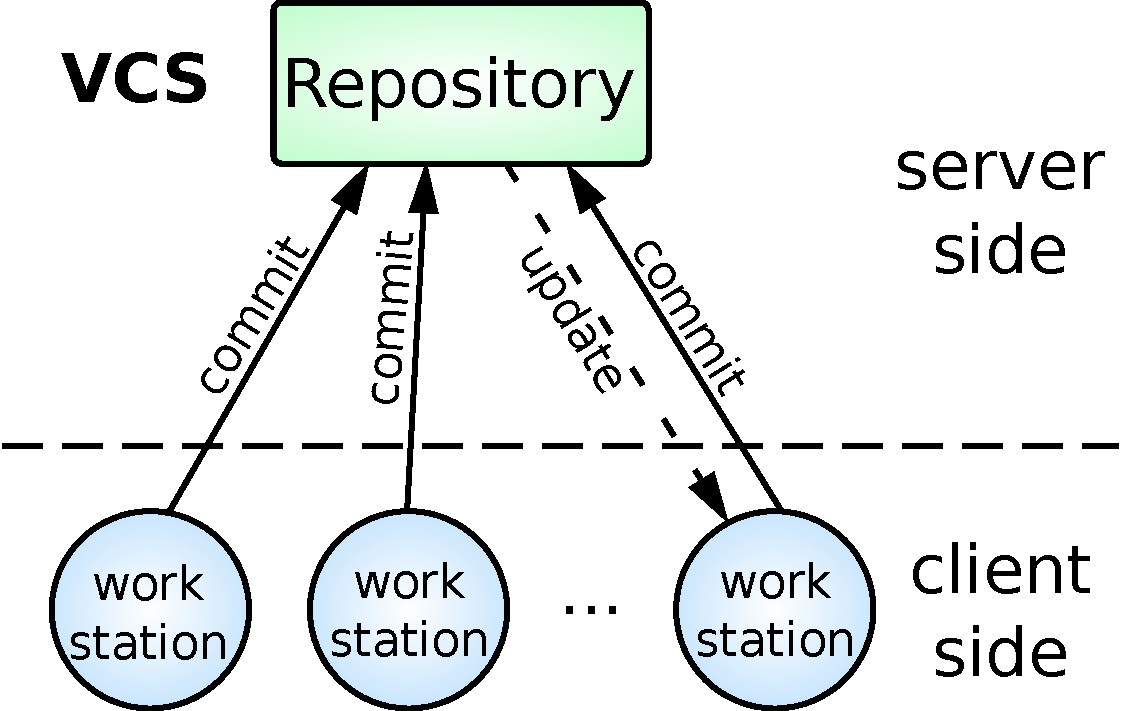
\includegraphics[height=0.40\textheight]{images/pdf/vcs.pdf}
     \ \\ \vspacing \vspacing \vspacing \vspacing
    \only<1>{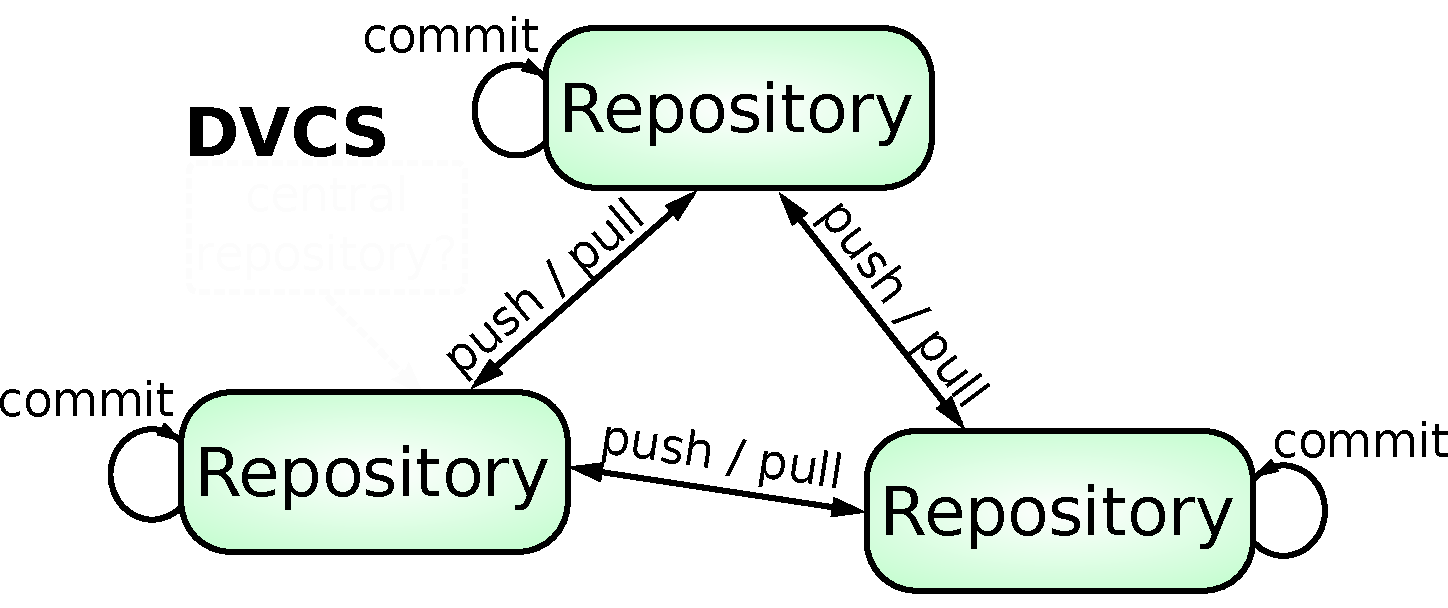
\includegraphics[height=0.35\textheight]{images/pdf/dvcs1.pdf}}
    \only<2>{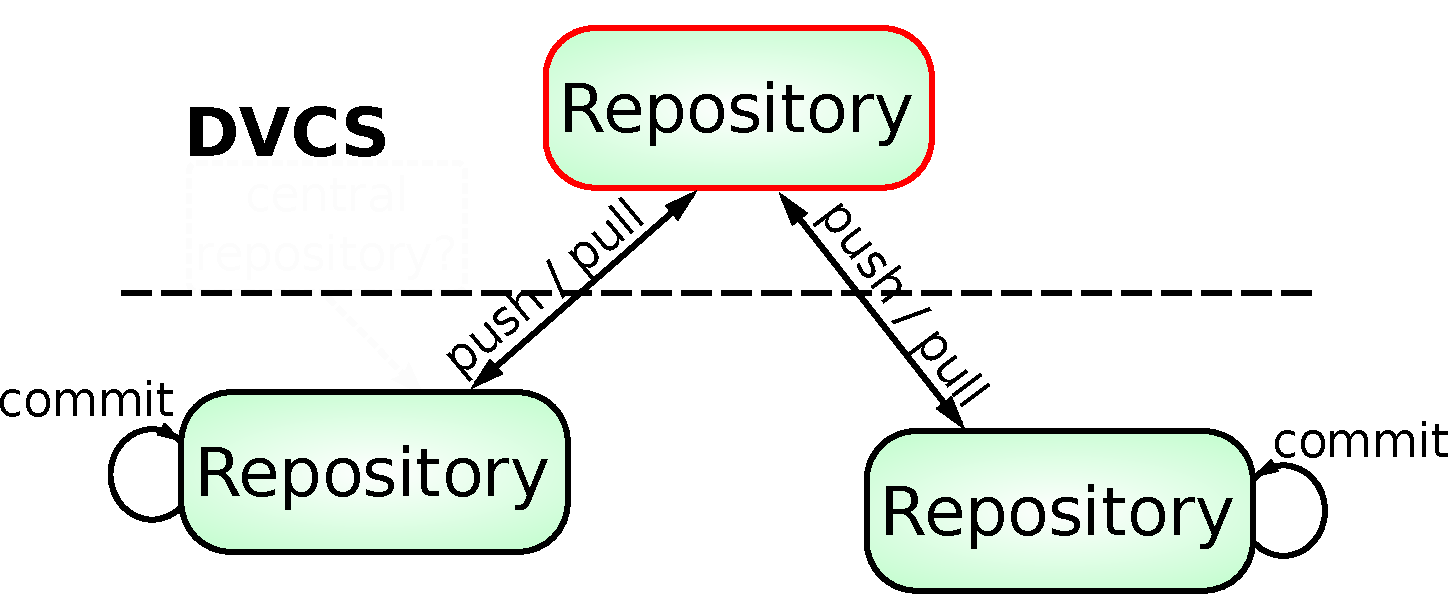
\includegraphics[height=0.35\textheight]{images/pdf/dvcs2.pdf}}
    \only<3>{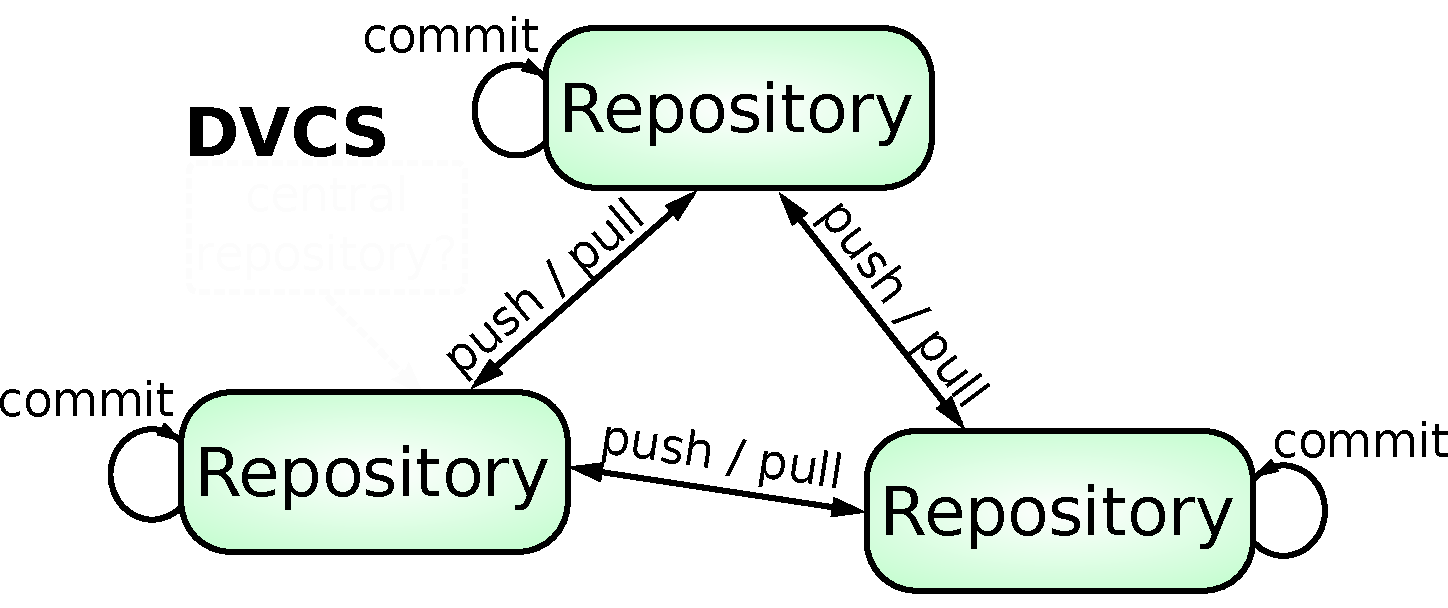
\includegraphics[height=0.35\textheight]{images/pdf/dvcs1.pdf}}
  \end{center}
\end{frame}

%%%%%%%%%%%%%%%%%%%%%%%%%%

\subsection{Advantages and disadvantages of DVCS}
\begin{frame}
  \frametitle{\insertsubsection}

  \begin{columns}[t]
    \column{.5\textwidth}
    \textbf{Advantages}
    \begin{itemize}
    \item Full repository in the local machine: full history,
      branches, work offline...
    \item Improves the \textit{workflow} for collaborative work
    \item Integration of changes from external sources
    \item Makes handling different versions for a project easier
    \item Better separation between private and public work
    \item Implicit \textit{back-up} copies
    \item Enables working offline
    \end{itemize}

    \column{.5\textwidth}
    \textbf{Disadvantages}
    \begin{itemize}
    \item More complex than \textit{VCS's}. Harder learning curve
    \item Initially cloning is slower (full repository cloning)
    \item Full clones can require more hard disk space
  \end{itemize}

  \end{columns}
\end{frame}

%%%%%%%%%%%%%%%%%%%%%%%%%%

\subsection{Subversion (VCS) vs Git (DVCS)}
\begin{frame}
  \frametitle{\insertsubsection}
  \begin{center}
    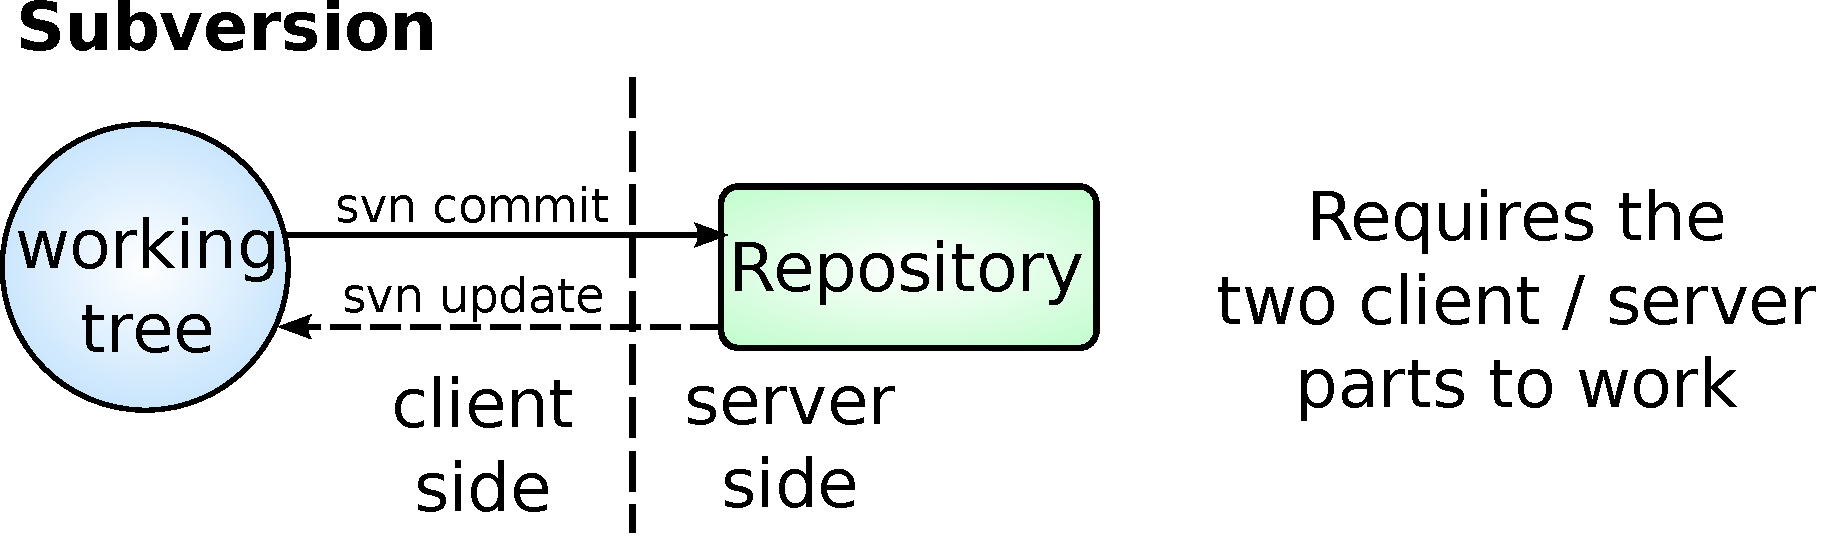
\includegraphics[height=0.30\textheight]{images/pdf/svn-layout.pdf}
     \ \\ \vspacing \vspacing \vspacing
    \only<1>{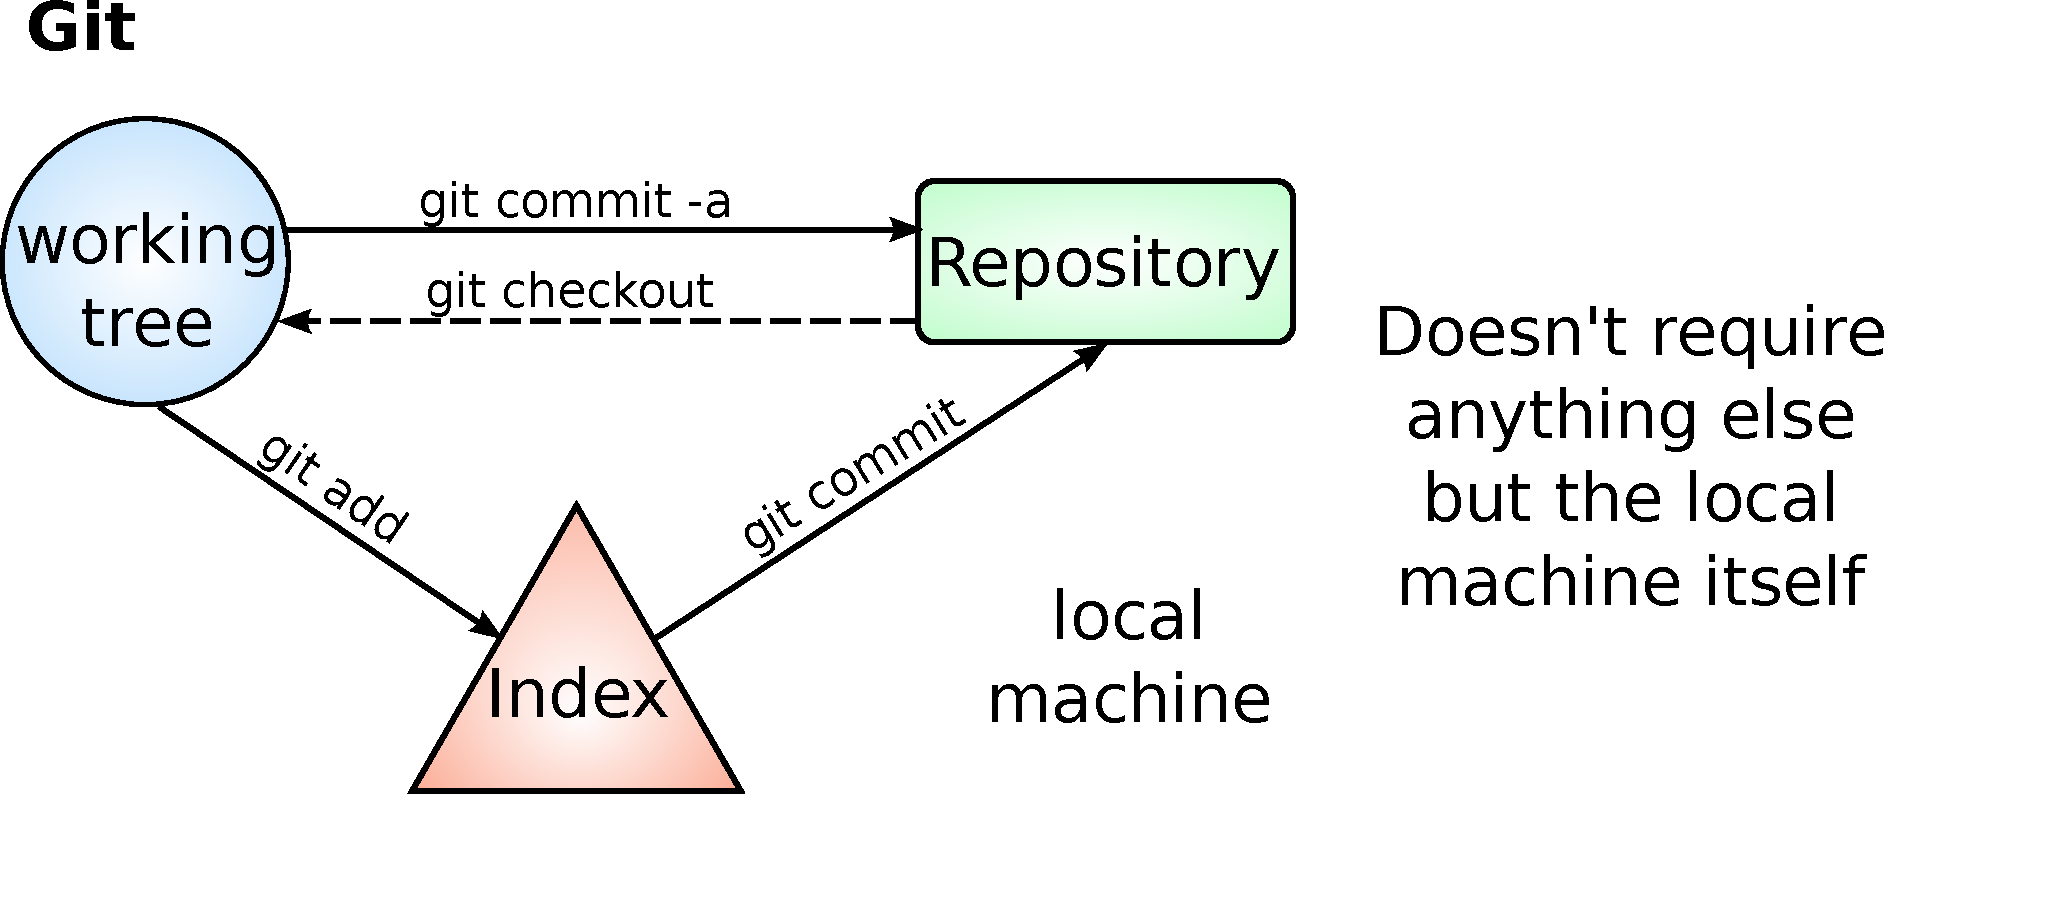
\includegraphics[height=0.50\textheight]{images/pdf/git-layout-solo.pdf}}
    \only<2>{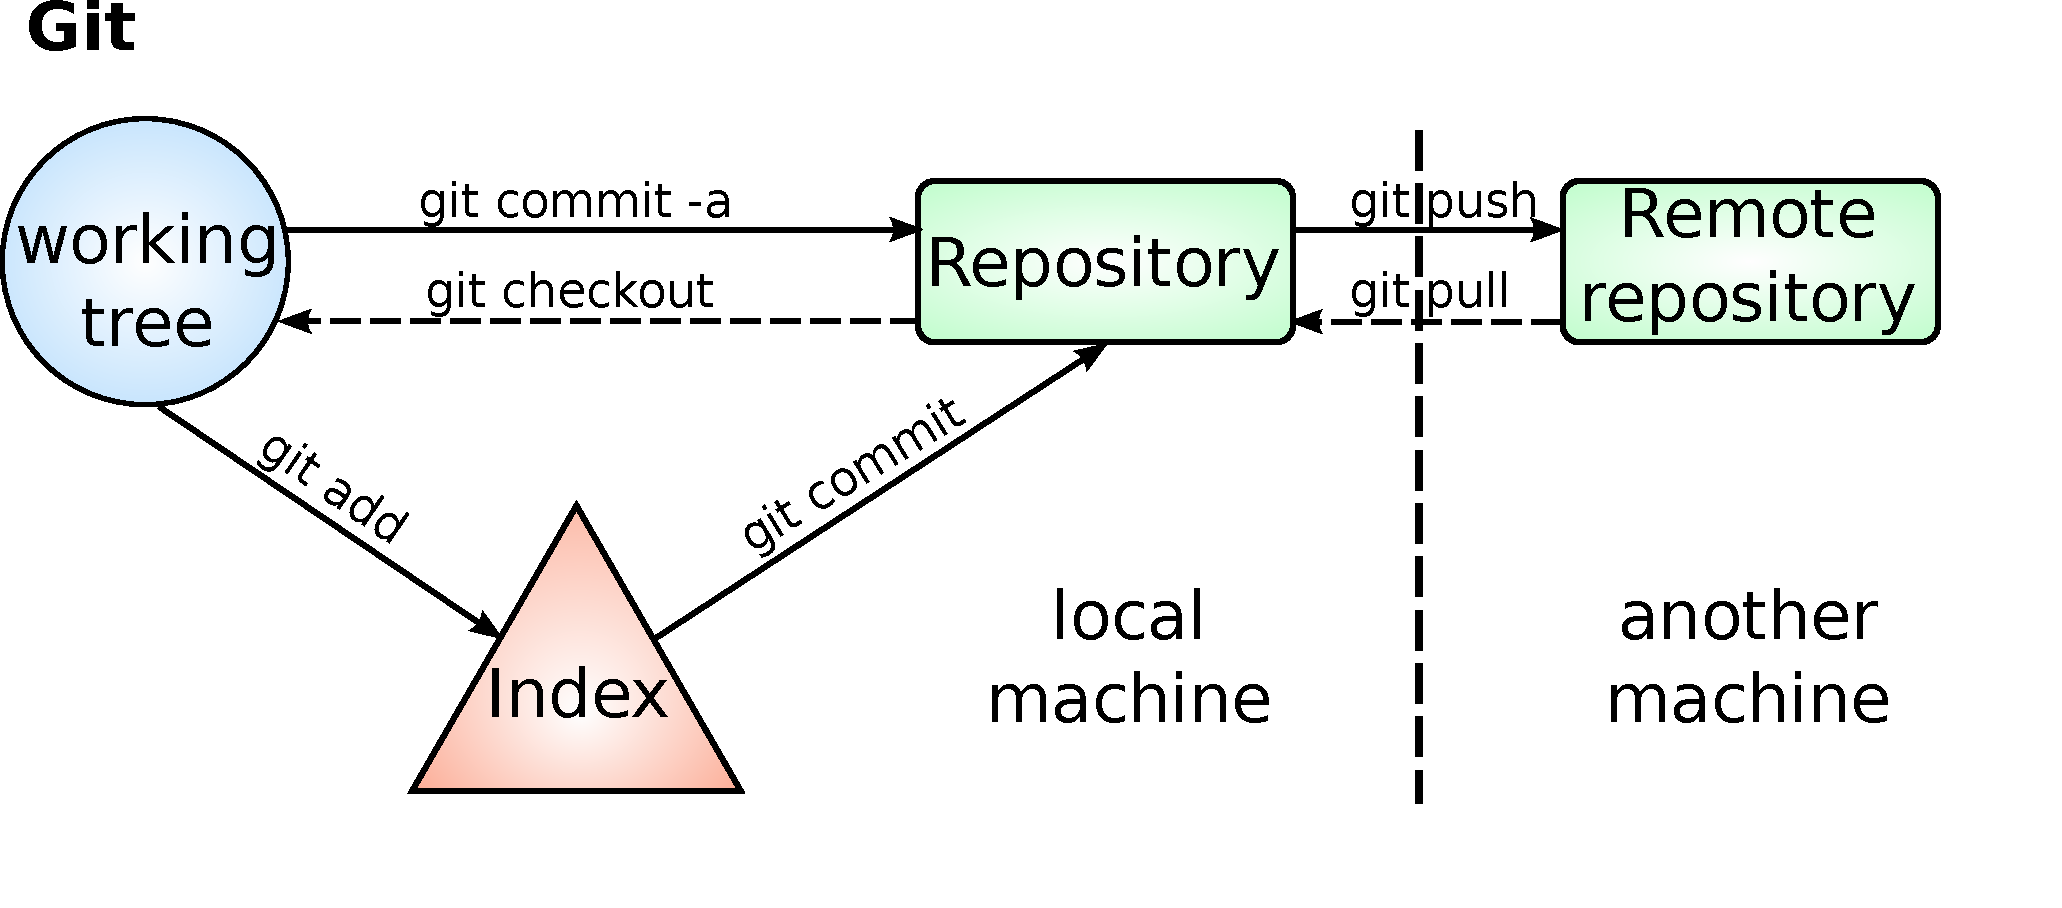
\includegraphics[height=0.50\textheight]{images/pdf/git-layout-remote.pdf}}
  \end{center}
\end{frame}

%%%%%%%%%%%%%%%%%%%%%%%%%%

\subsection{Typical workflow in git}
\begin{frame}
  \frametitle{\insertsubsection}
  \begin{center}
    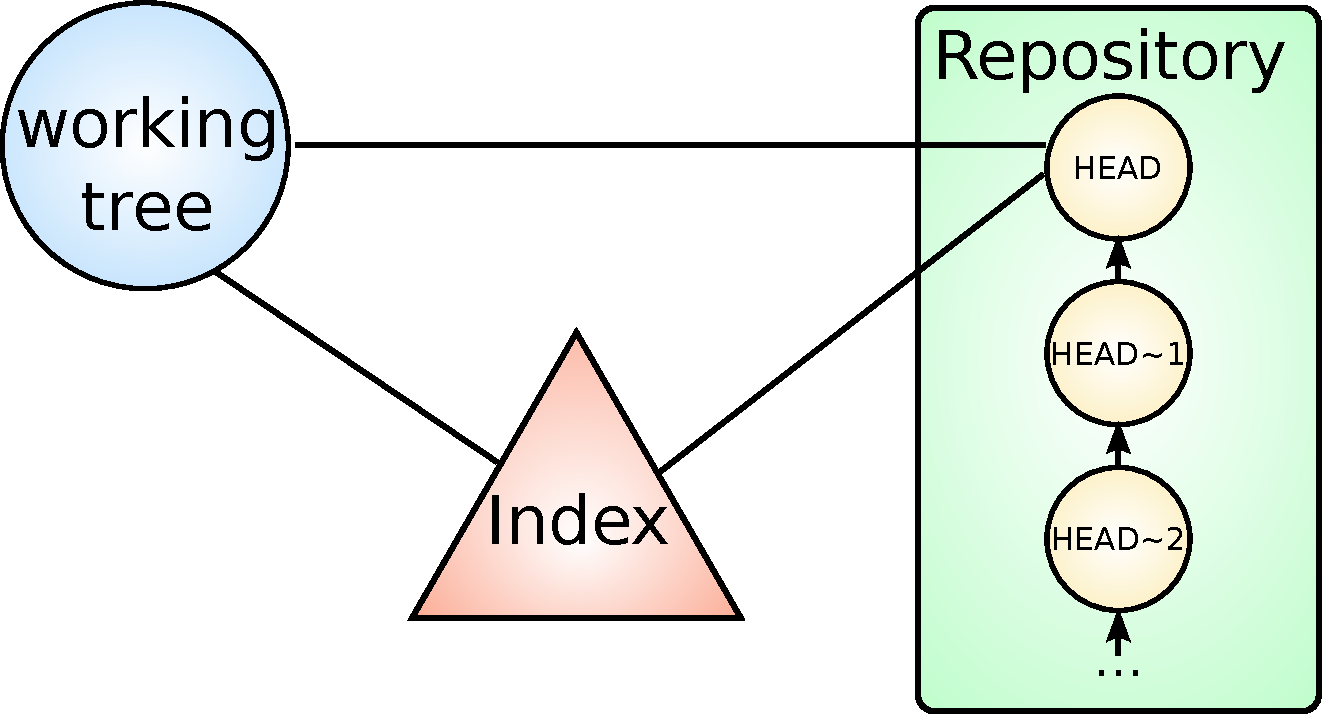
\includegraphics[width=1.0\textwidth]{images/pdf/git-detailed-1.pdf}
  \end{center}
\end{frame}
\begin{frame}
  \frametitle{\insertsubsection}
  \begin{center}
    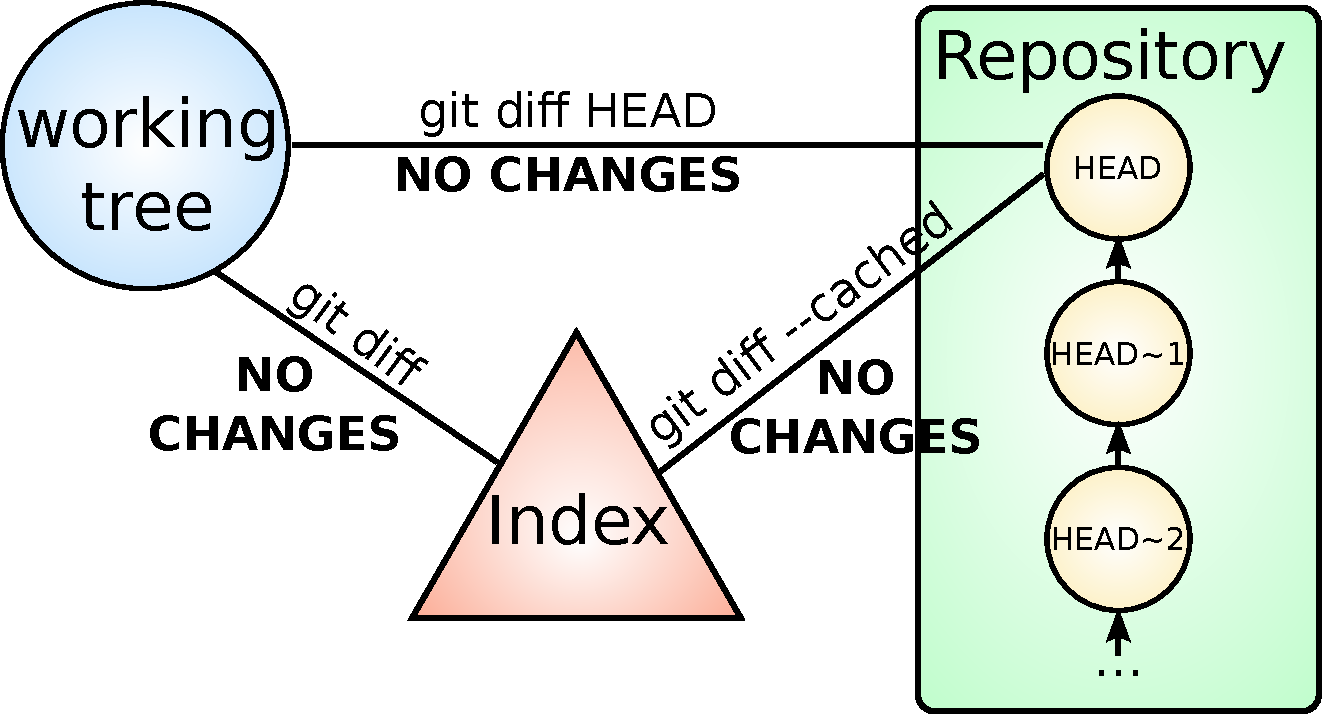
\includegraphics[width=1.0\textwidth]{images/pdf/git-detailed-2.pdf}
  \end{center}
\end{frame}
\begin{frame}
  \frametitle{\insertsubsection}
  \begin{center}
    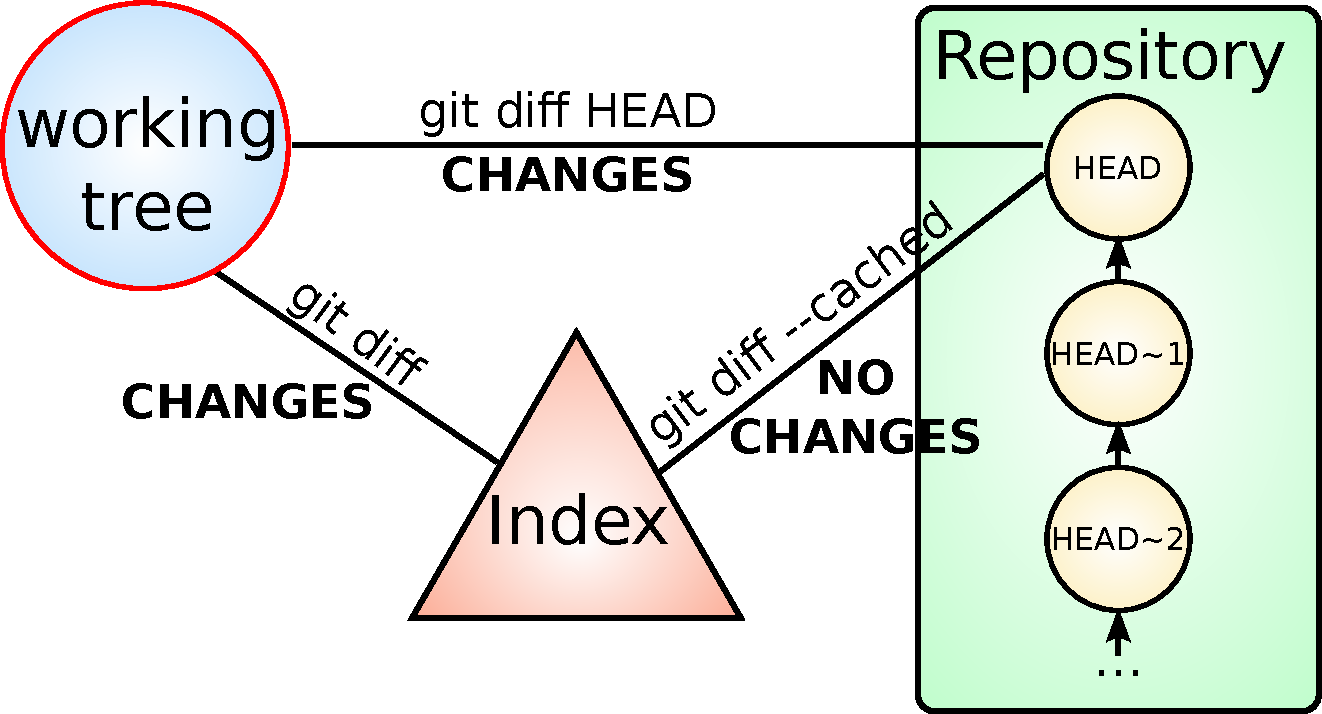
\includegraphics[width=1.0\textwidth]{images/pdf/git-detailed-3.pdf}
  \end{center}
\end{frame}
\begin{frame}
  \frametitle{\insertsubsection}
  \begin{center}
    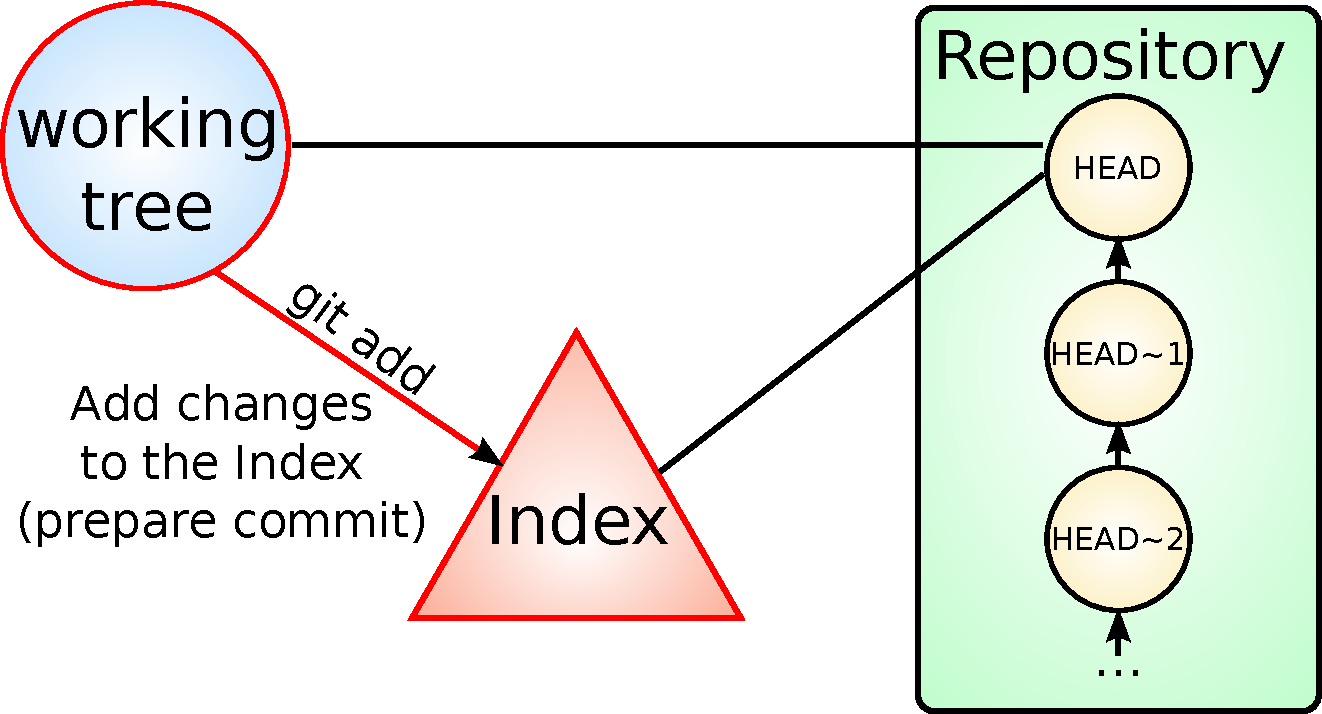
\includegraphics[width=1.0\textwidth]{images/pdf/git-detailed-4.pdf}
  \end{center}
\end{frame}
\begin{frame}
  \frametitle{\insertsubsection}
  \begin{center}
    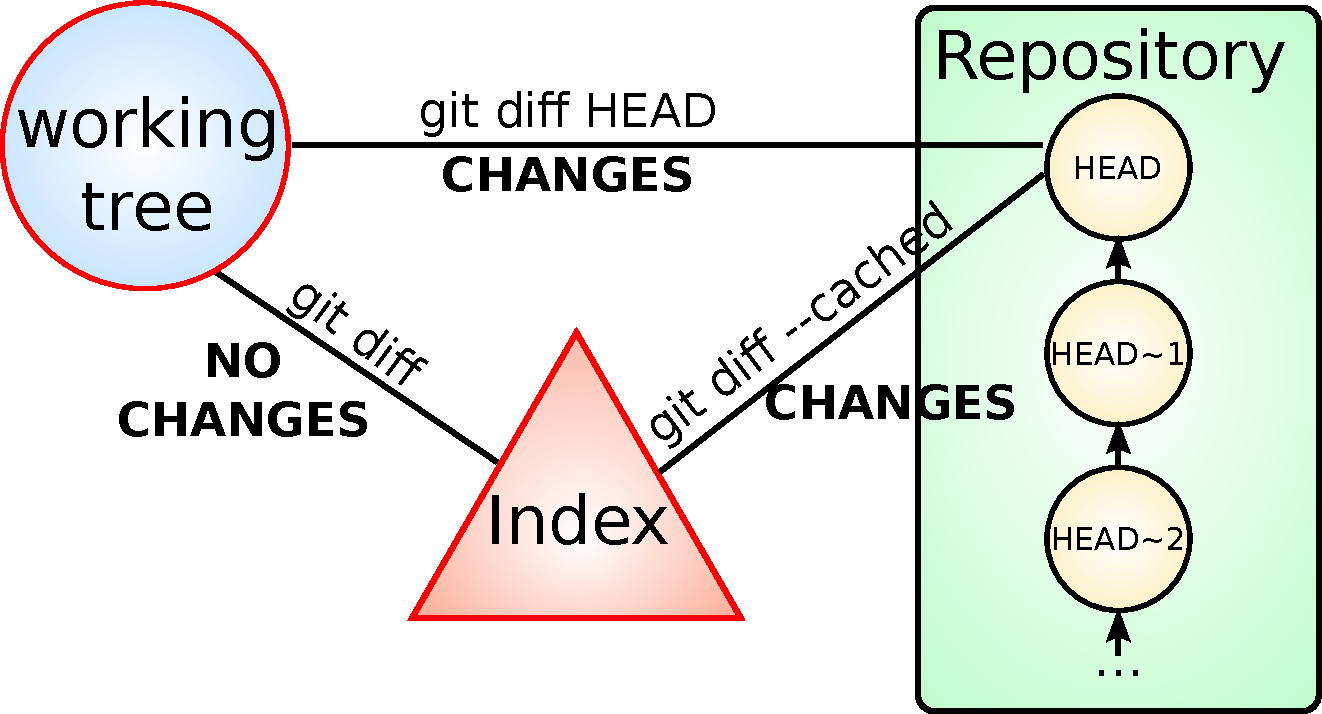
\includegraphics[width=1.0\textwidth]{images/pdf/git-detailed-5.pdf}
  \end{center}
\end{frame}
\begin{frame}
  \frametitle{\insertsubsection}
  \begin{center}
    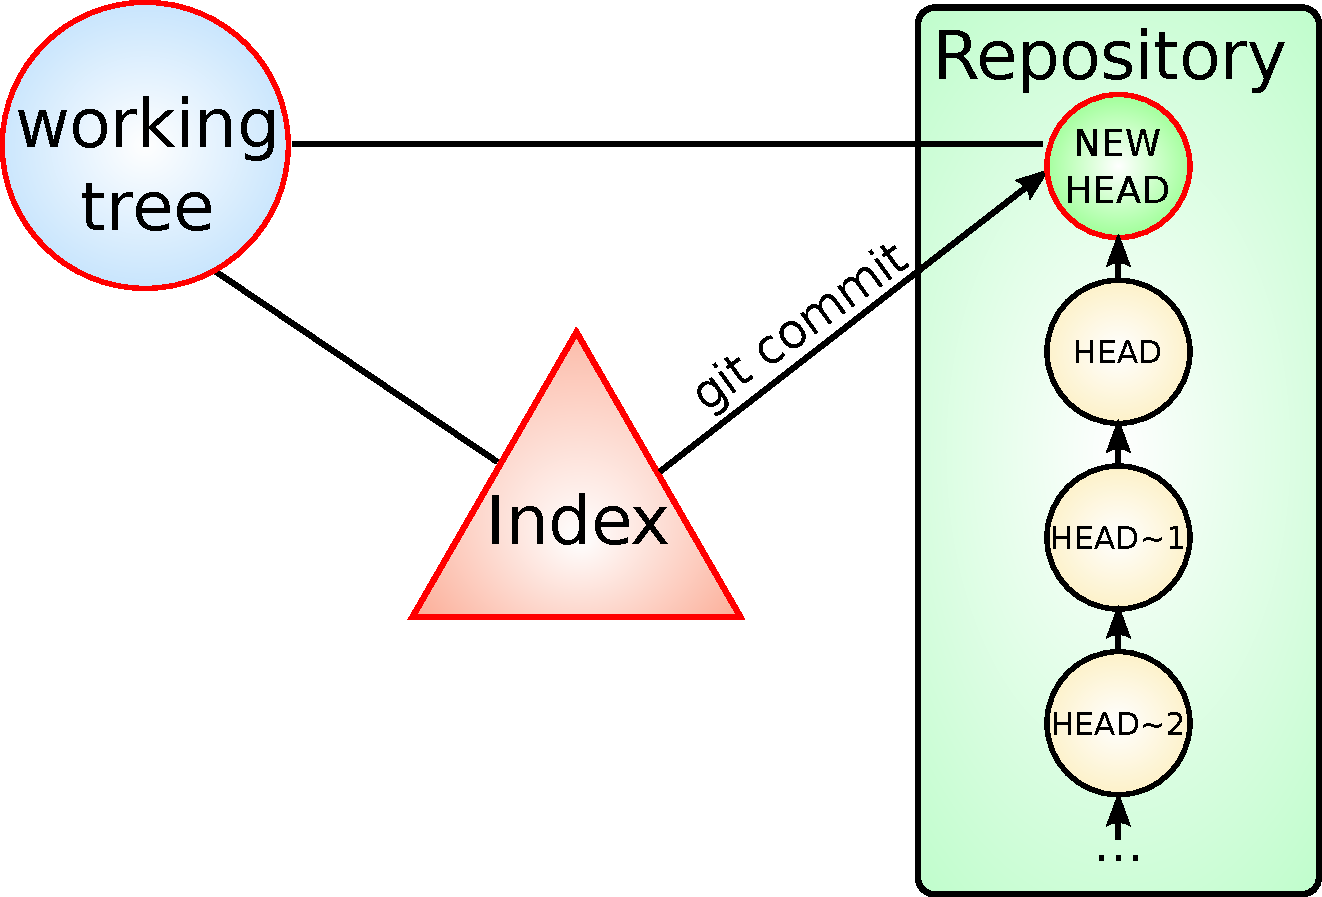
\includegraphics[width=1.0\textwidth]{images/pdf/git-detailed-6.pdf}
  \end{center}
\end{frame}
\begin{frame}
  \frametitle{\insertsubsection}
  \begin{center}
    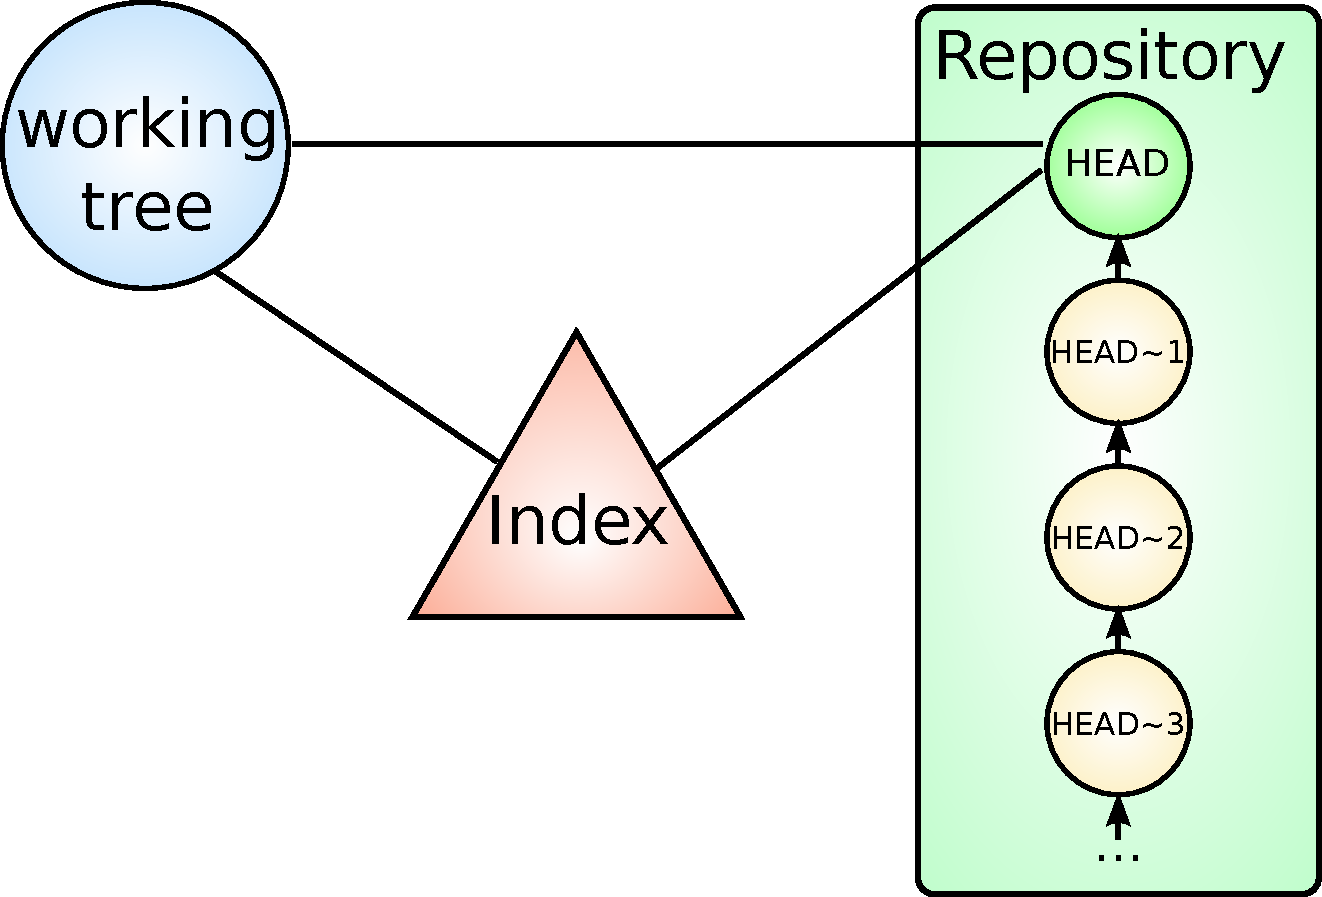
\includegraphics[width=1.0\textwidth]{images/pdf/git-detailed-7.pdf}
  \end{center}
\end{frame}
\begin{frame}
  \frametitle{\insertsubsection}
  \begin{center}
    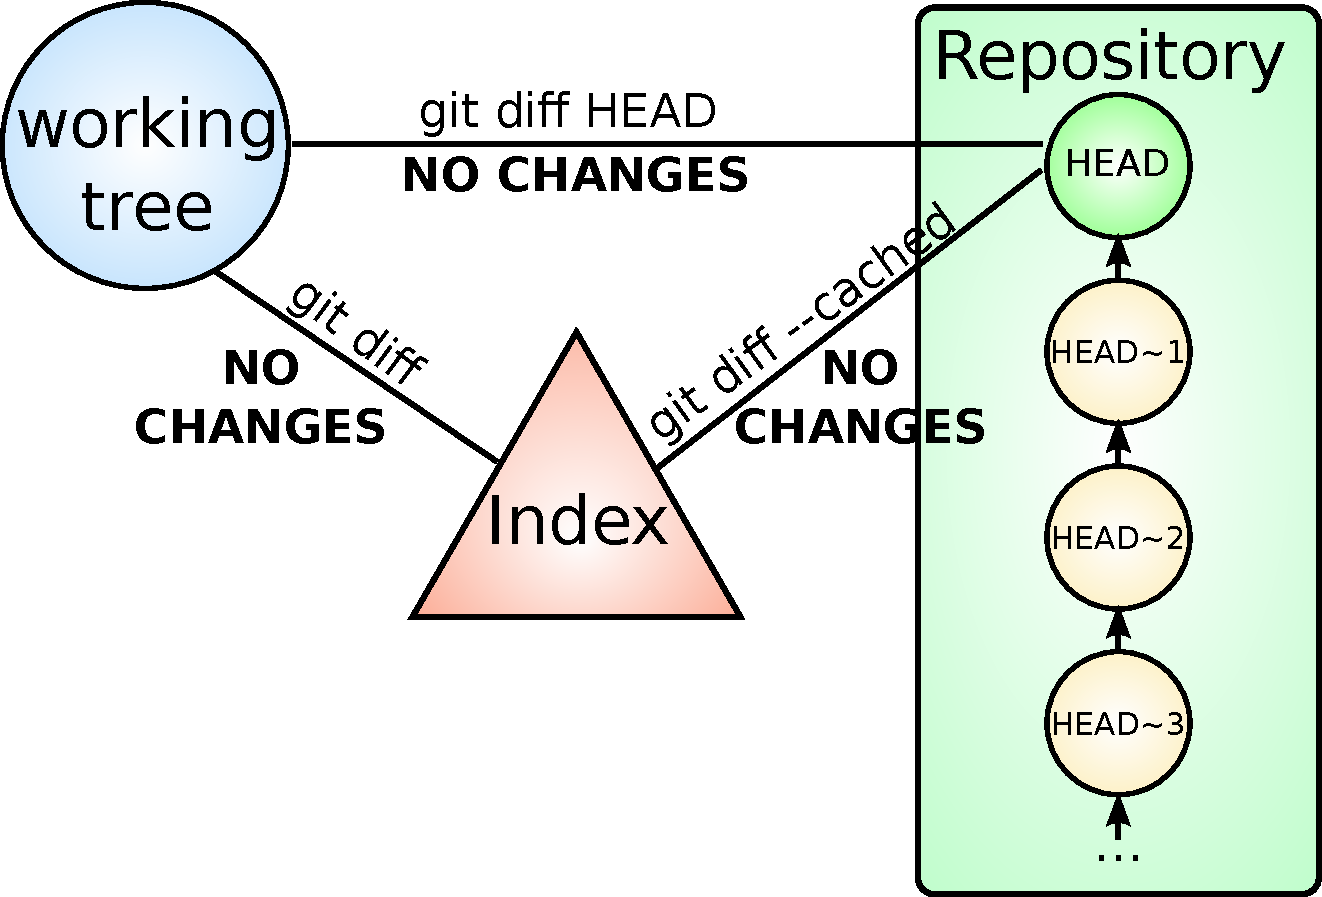
\includegraphics[width=1.0\textwidth]{images/pdf/git-detailed-8.pdf}
  \end{center}
\end{frame}
\begin{frame}
  \frametitle{\insertsubsection}
  \begin{center}
    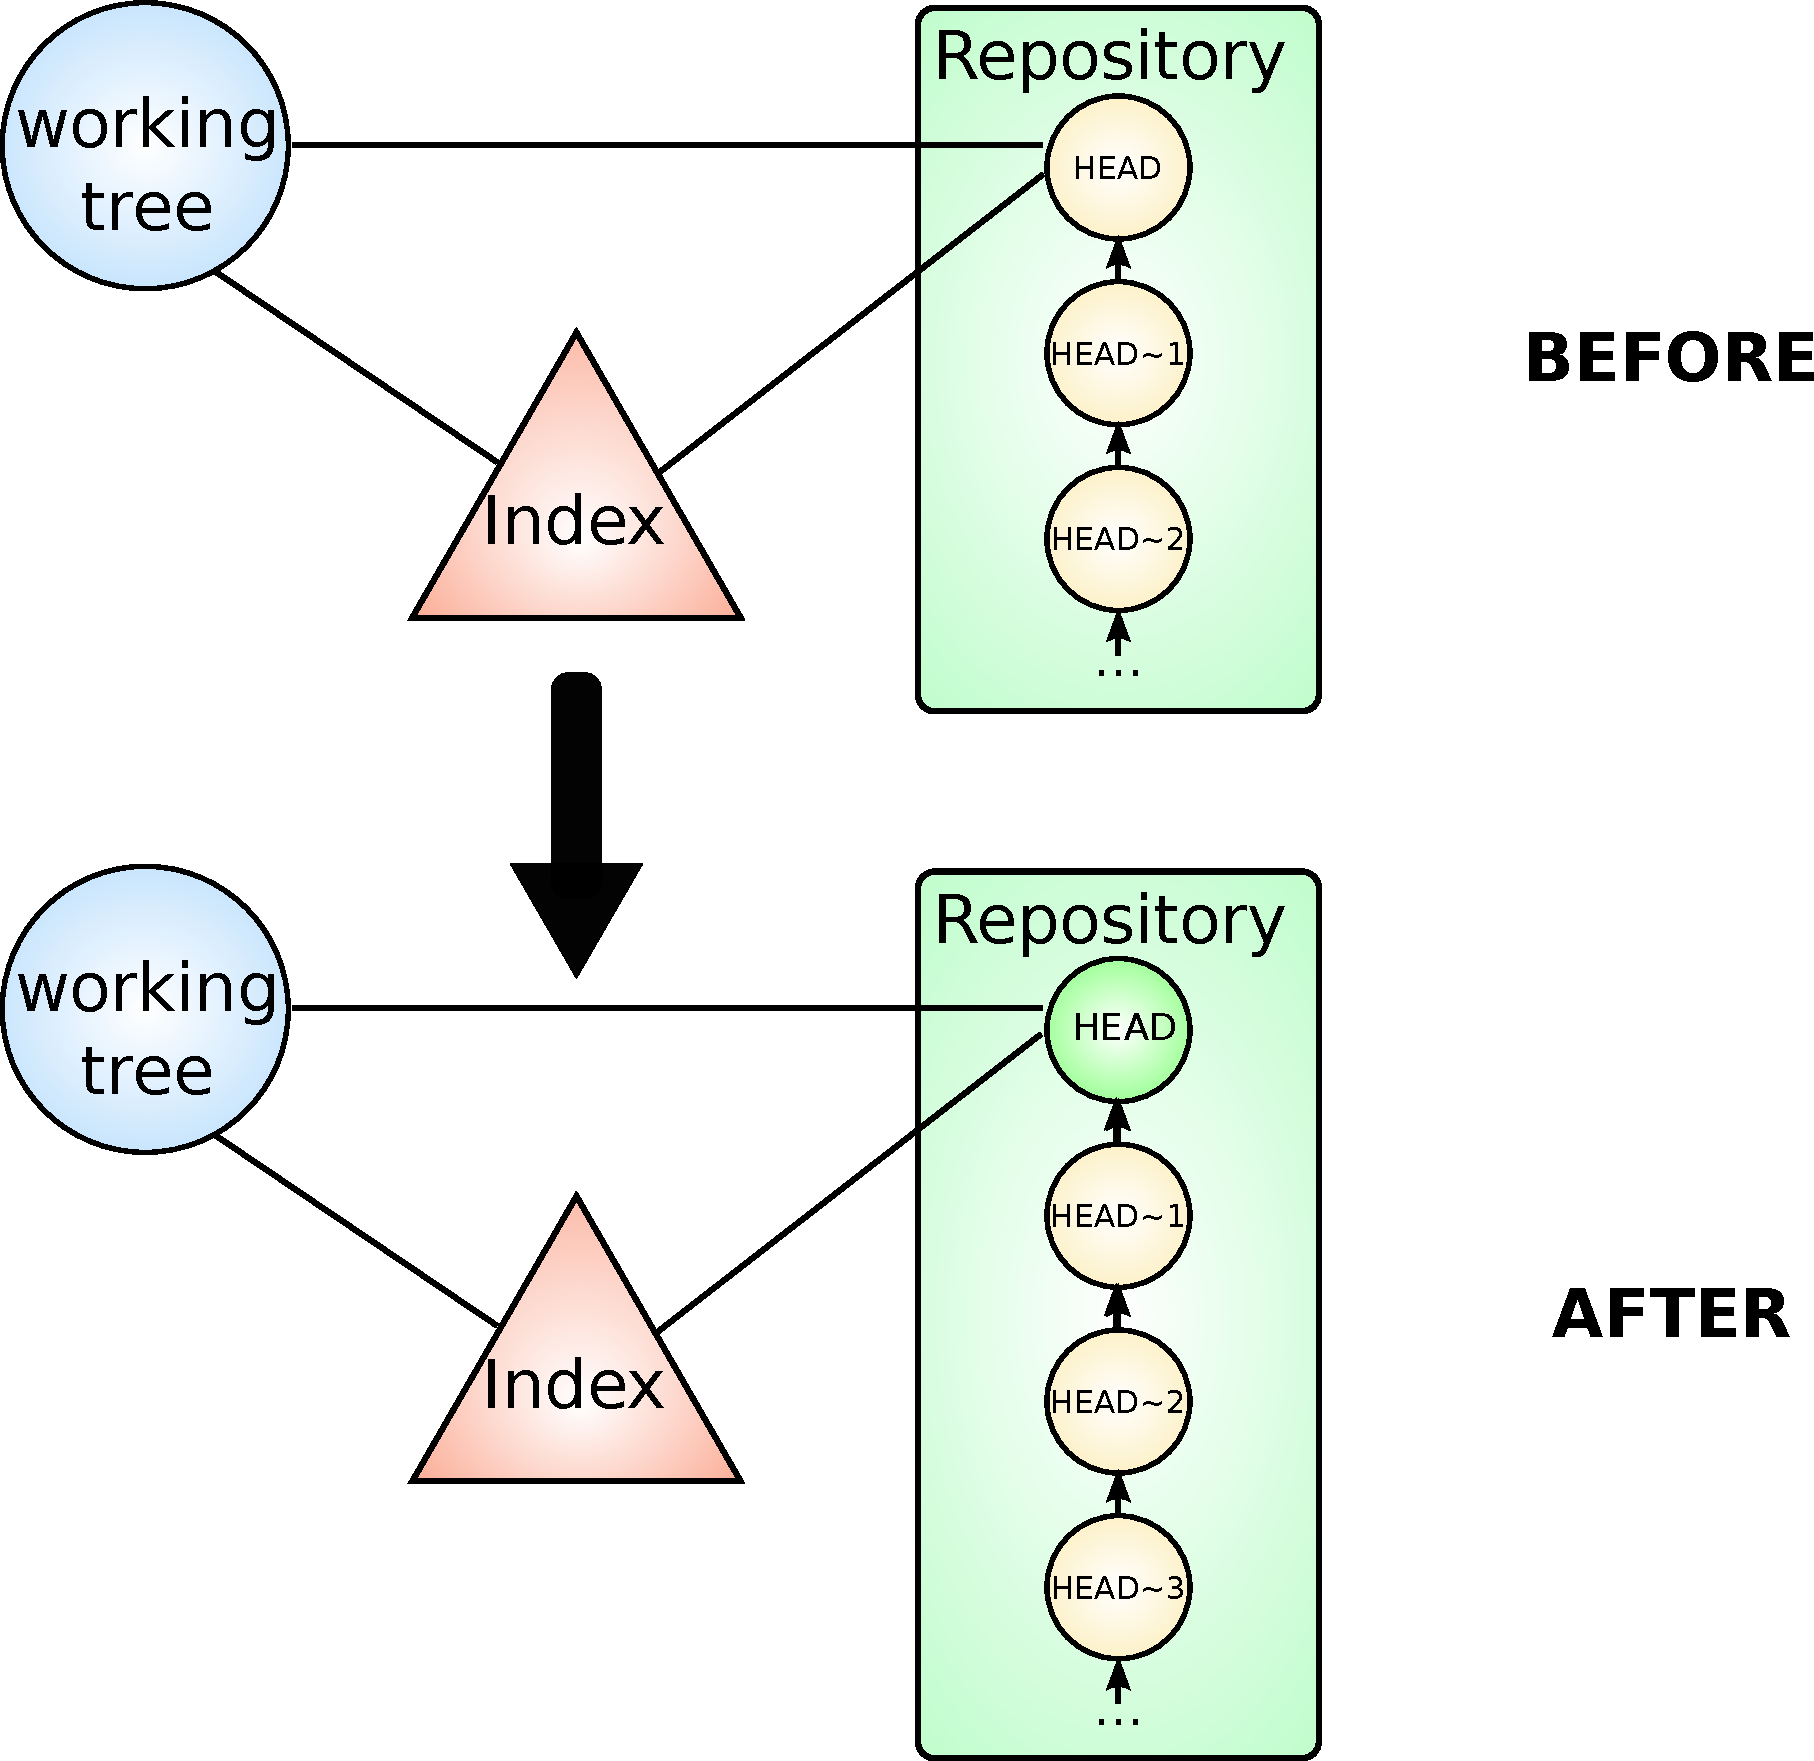
\includegraphics[height=0.8\textheight]{images/pdf/git-detailed-9.pdf}
  \end{center}
\end{frame}

%%%%%%%%%%%%%%%%%%%%%%%%%%

\subsection{Typical workflow in git - git push}
\begin{frame}
  \frametitle{\insertsubsection}
  \begin{center}
    \only<1>{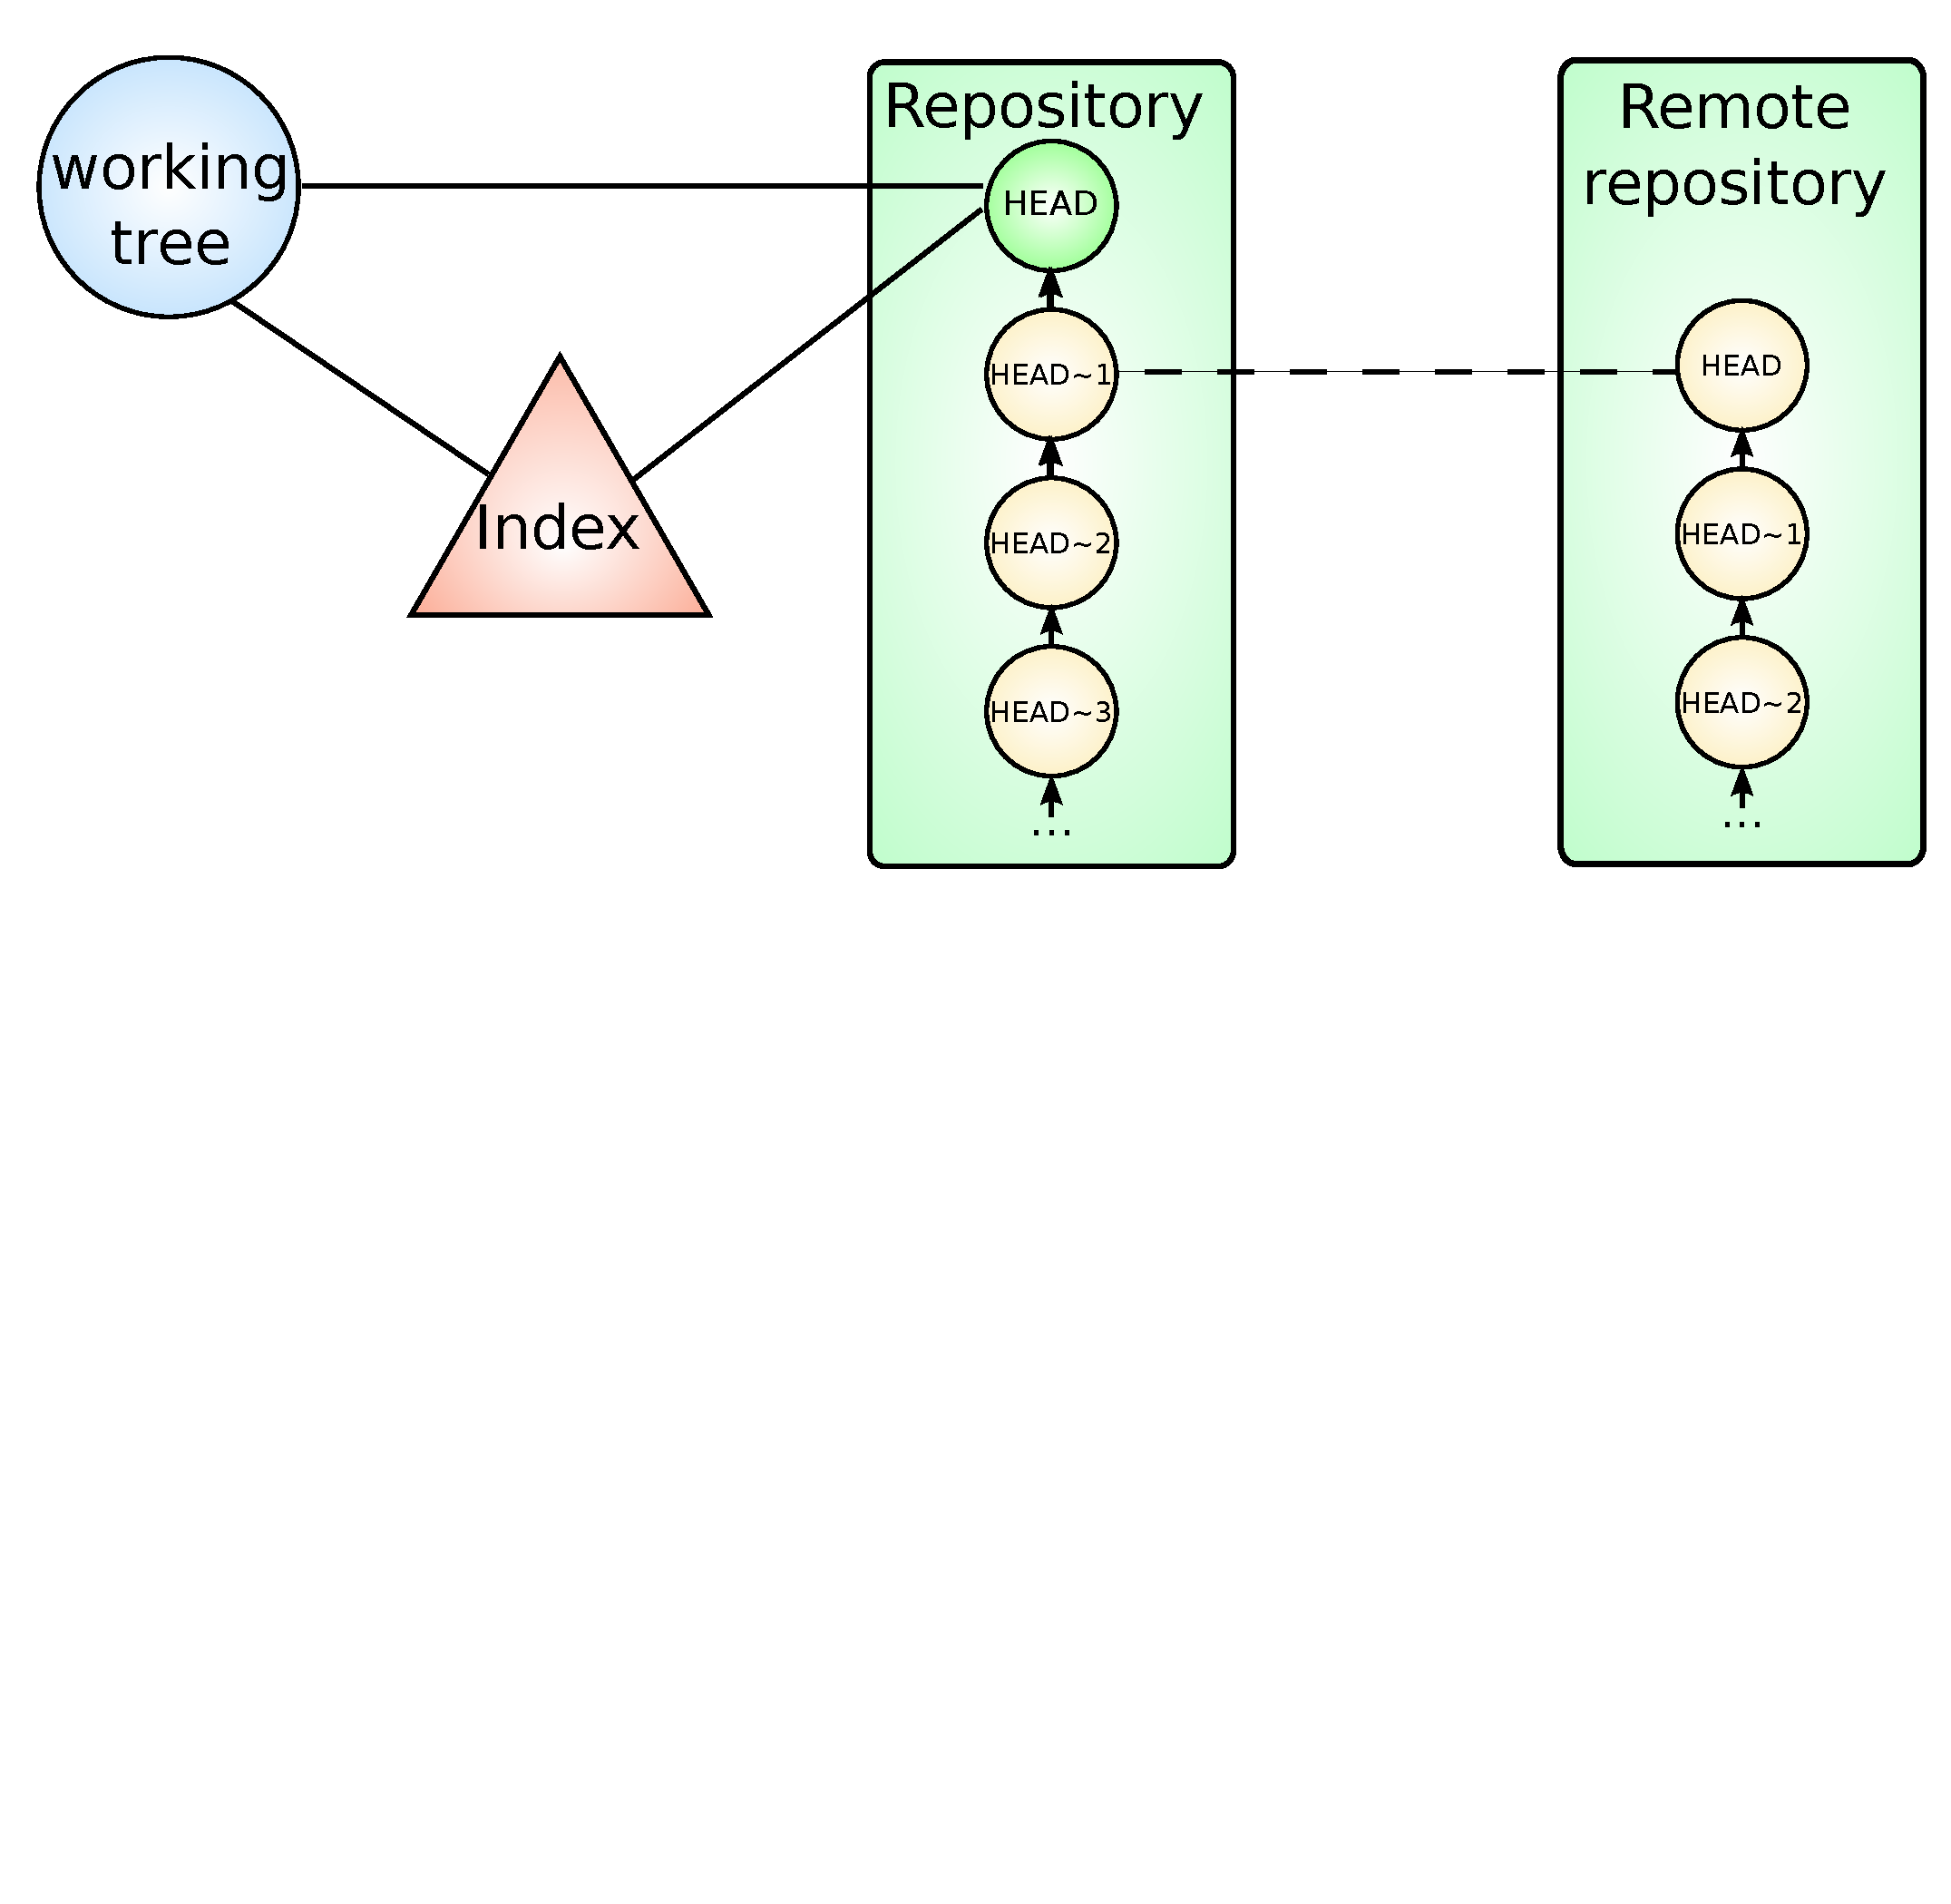
\includegraphics[height=0.8\textheight]{images/pdf/git-detailed-10.pdf}}
    \only<2>{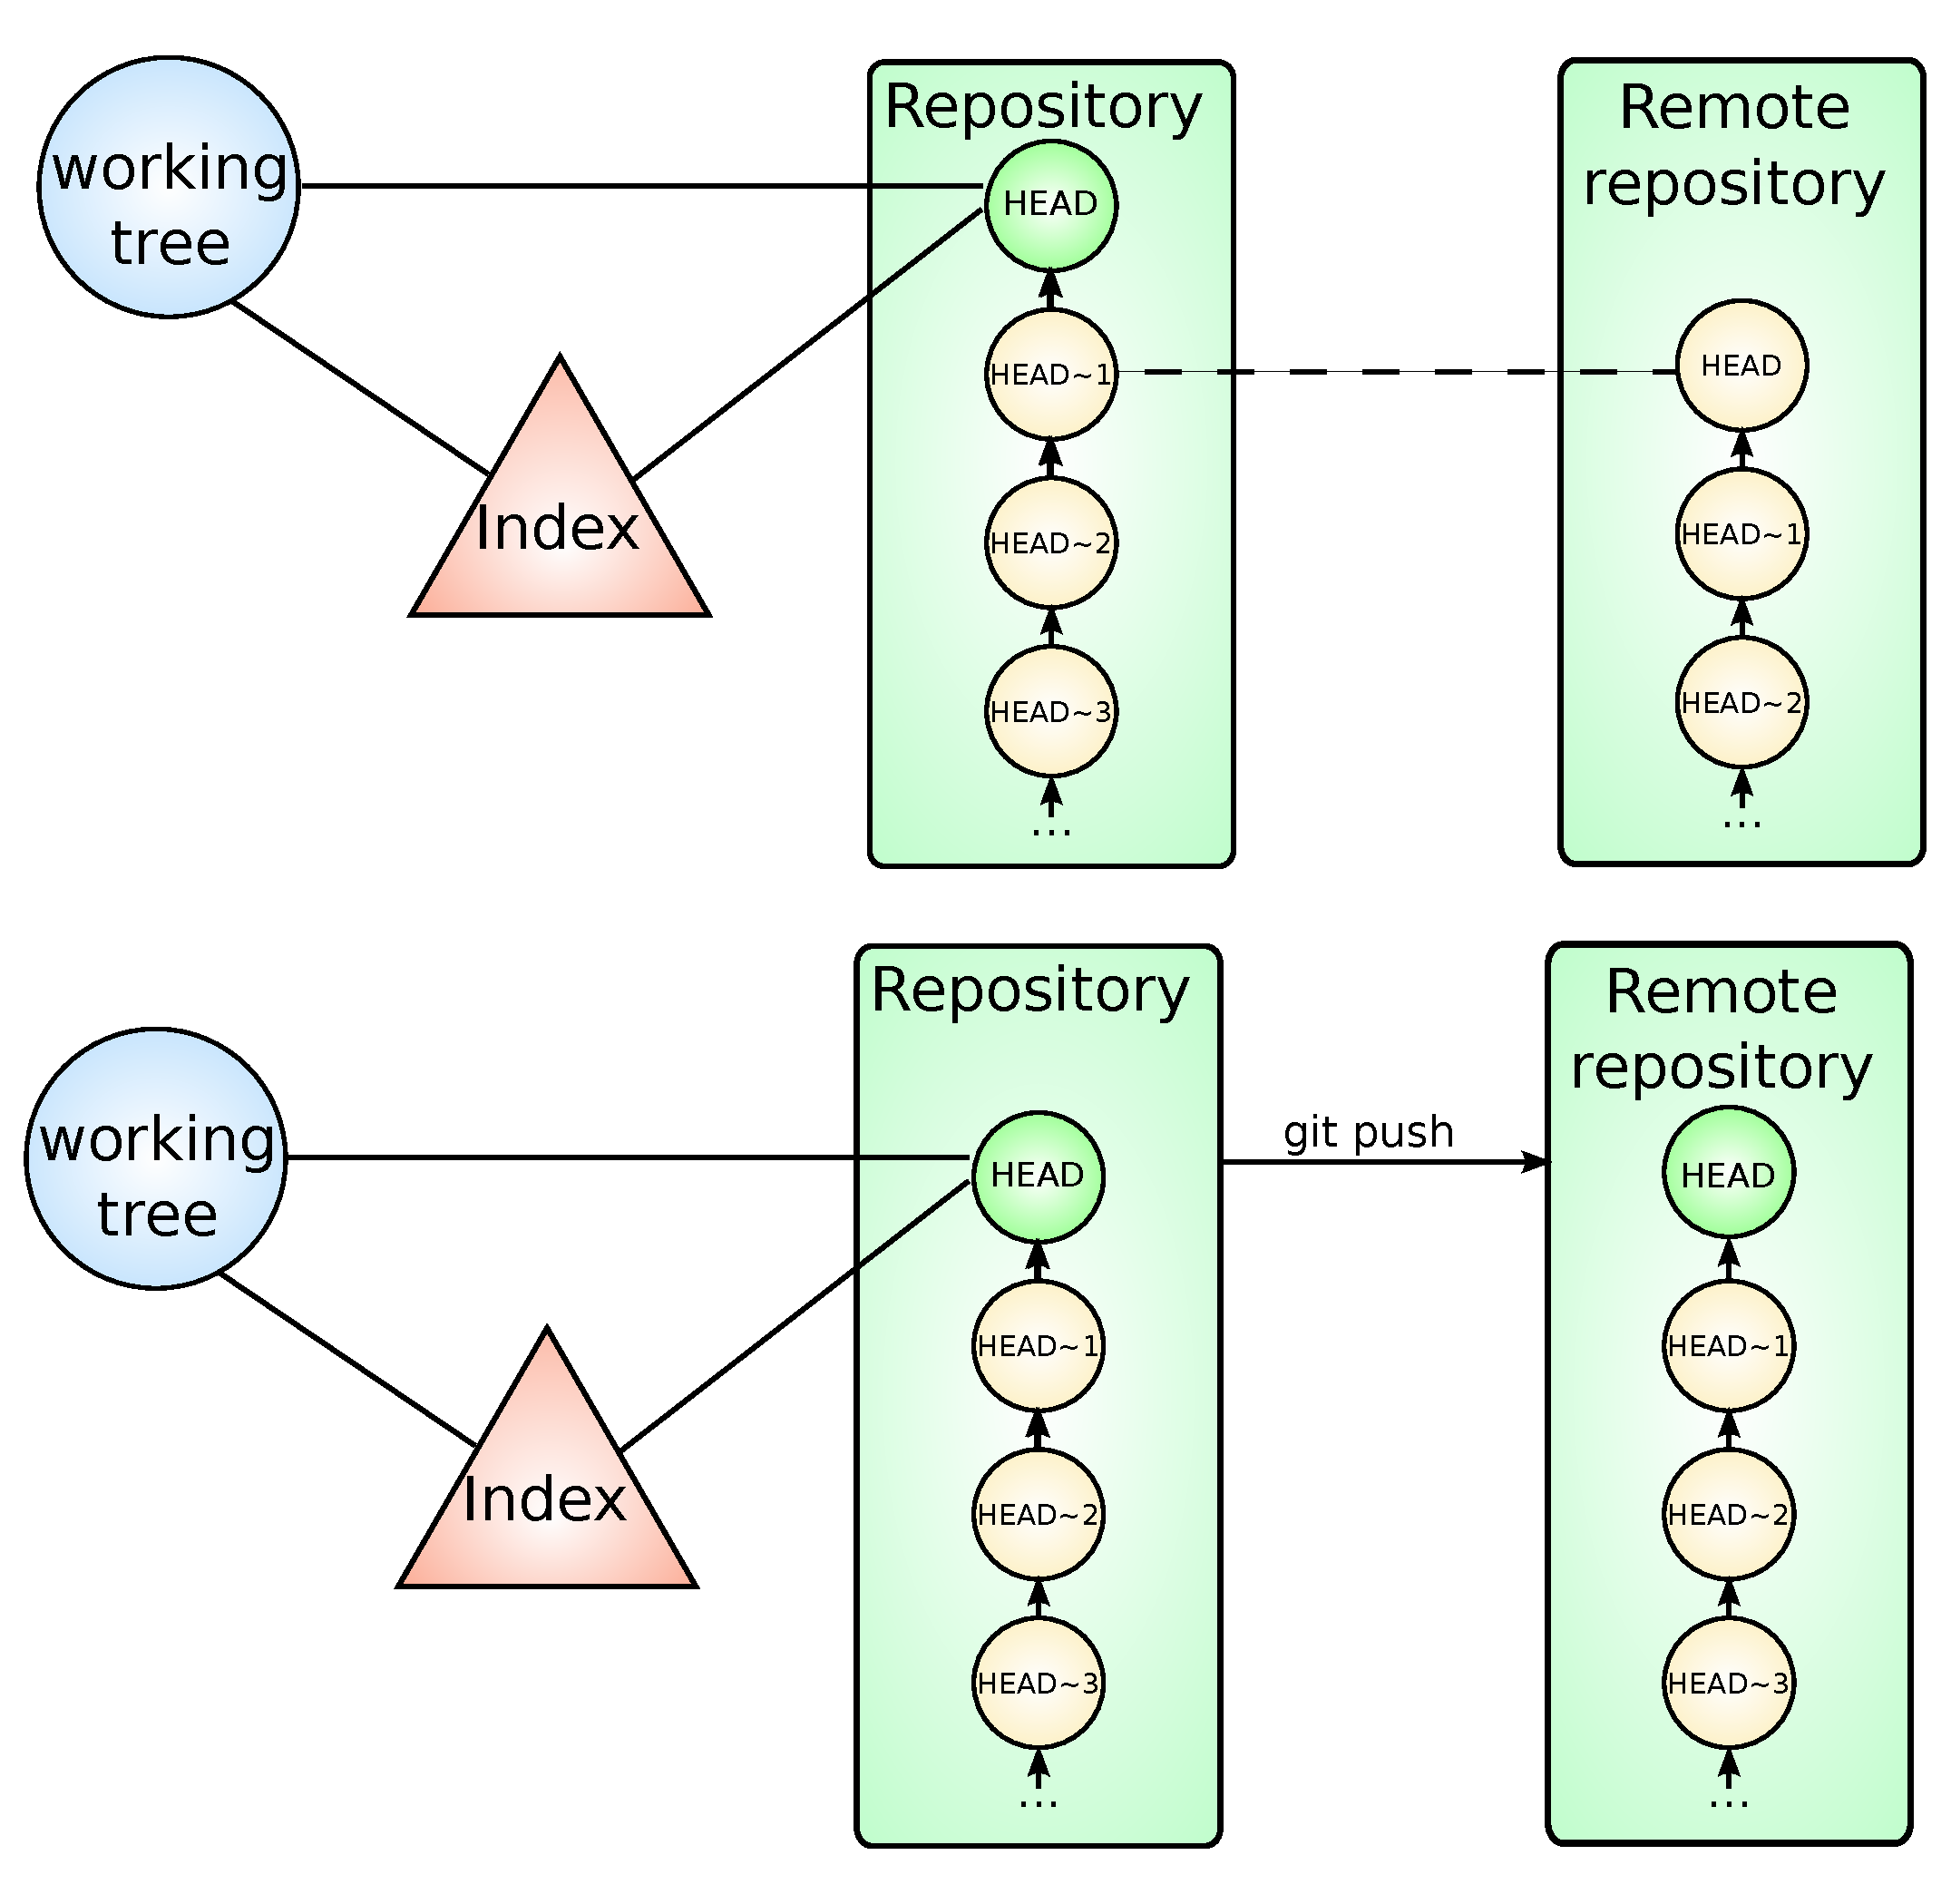
\includegraphics[height=0.8\textheight]{images/pdf/git-detailed-11.pdf}}
  \end{center}
\end{frame}

%%%%%%%%%%%%%%%%%%%%%%%%%%

\subsection{Typical workflow in git - git pull}
\begin{frame}
  \frametitle{\insertsubsection}
  \begin{center}
    \only<1>{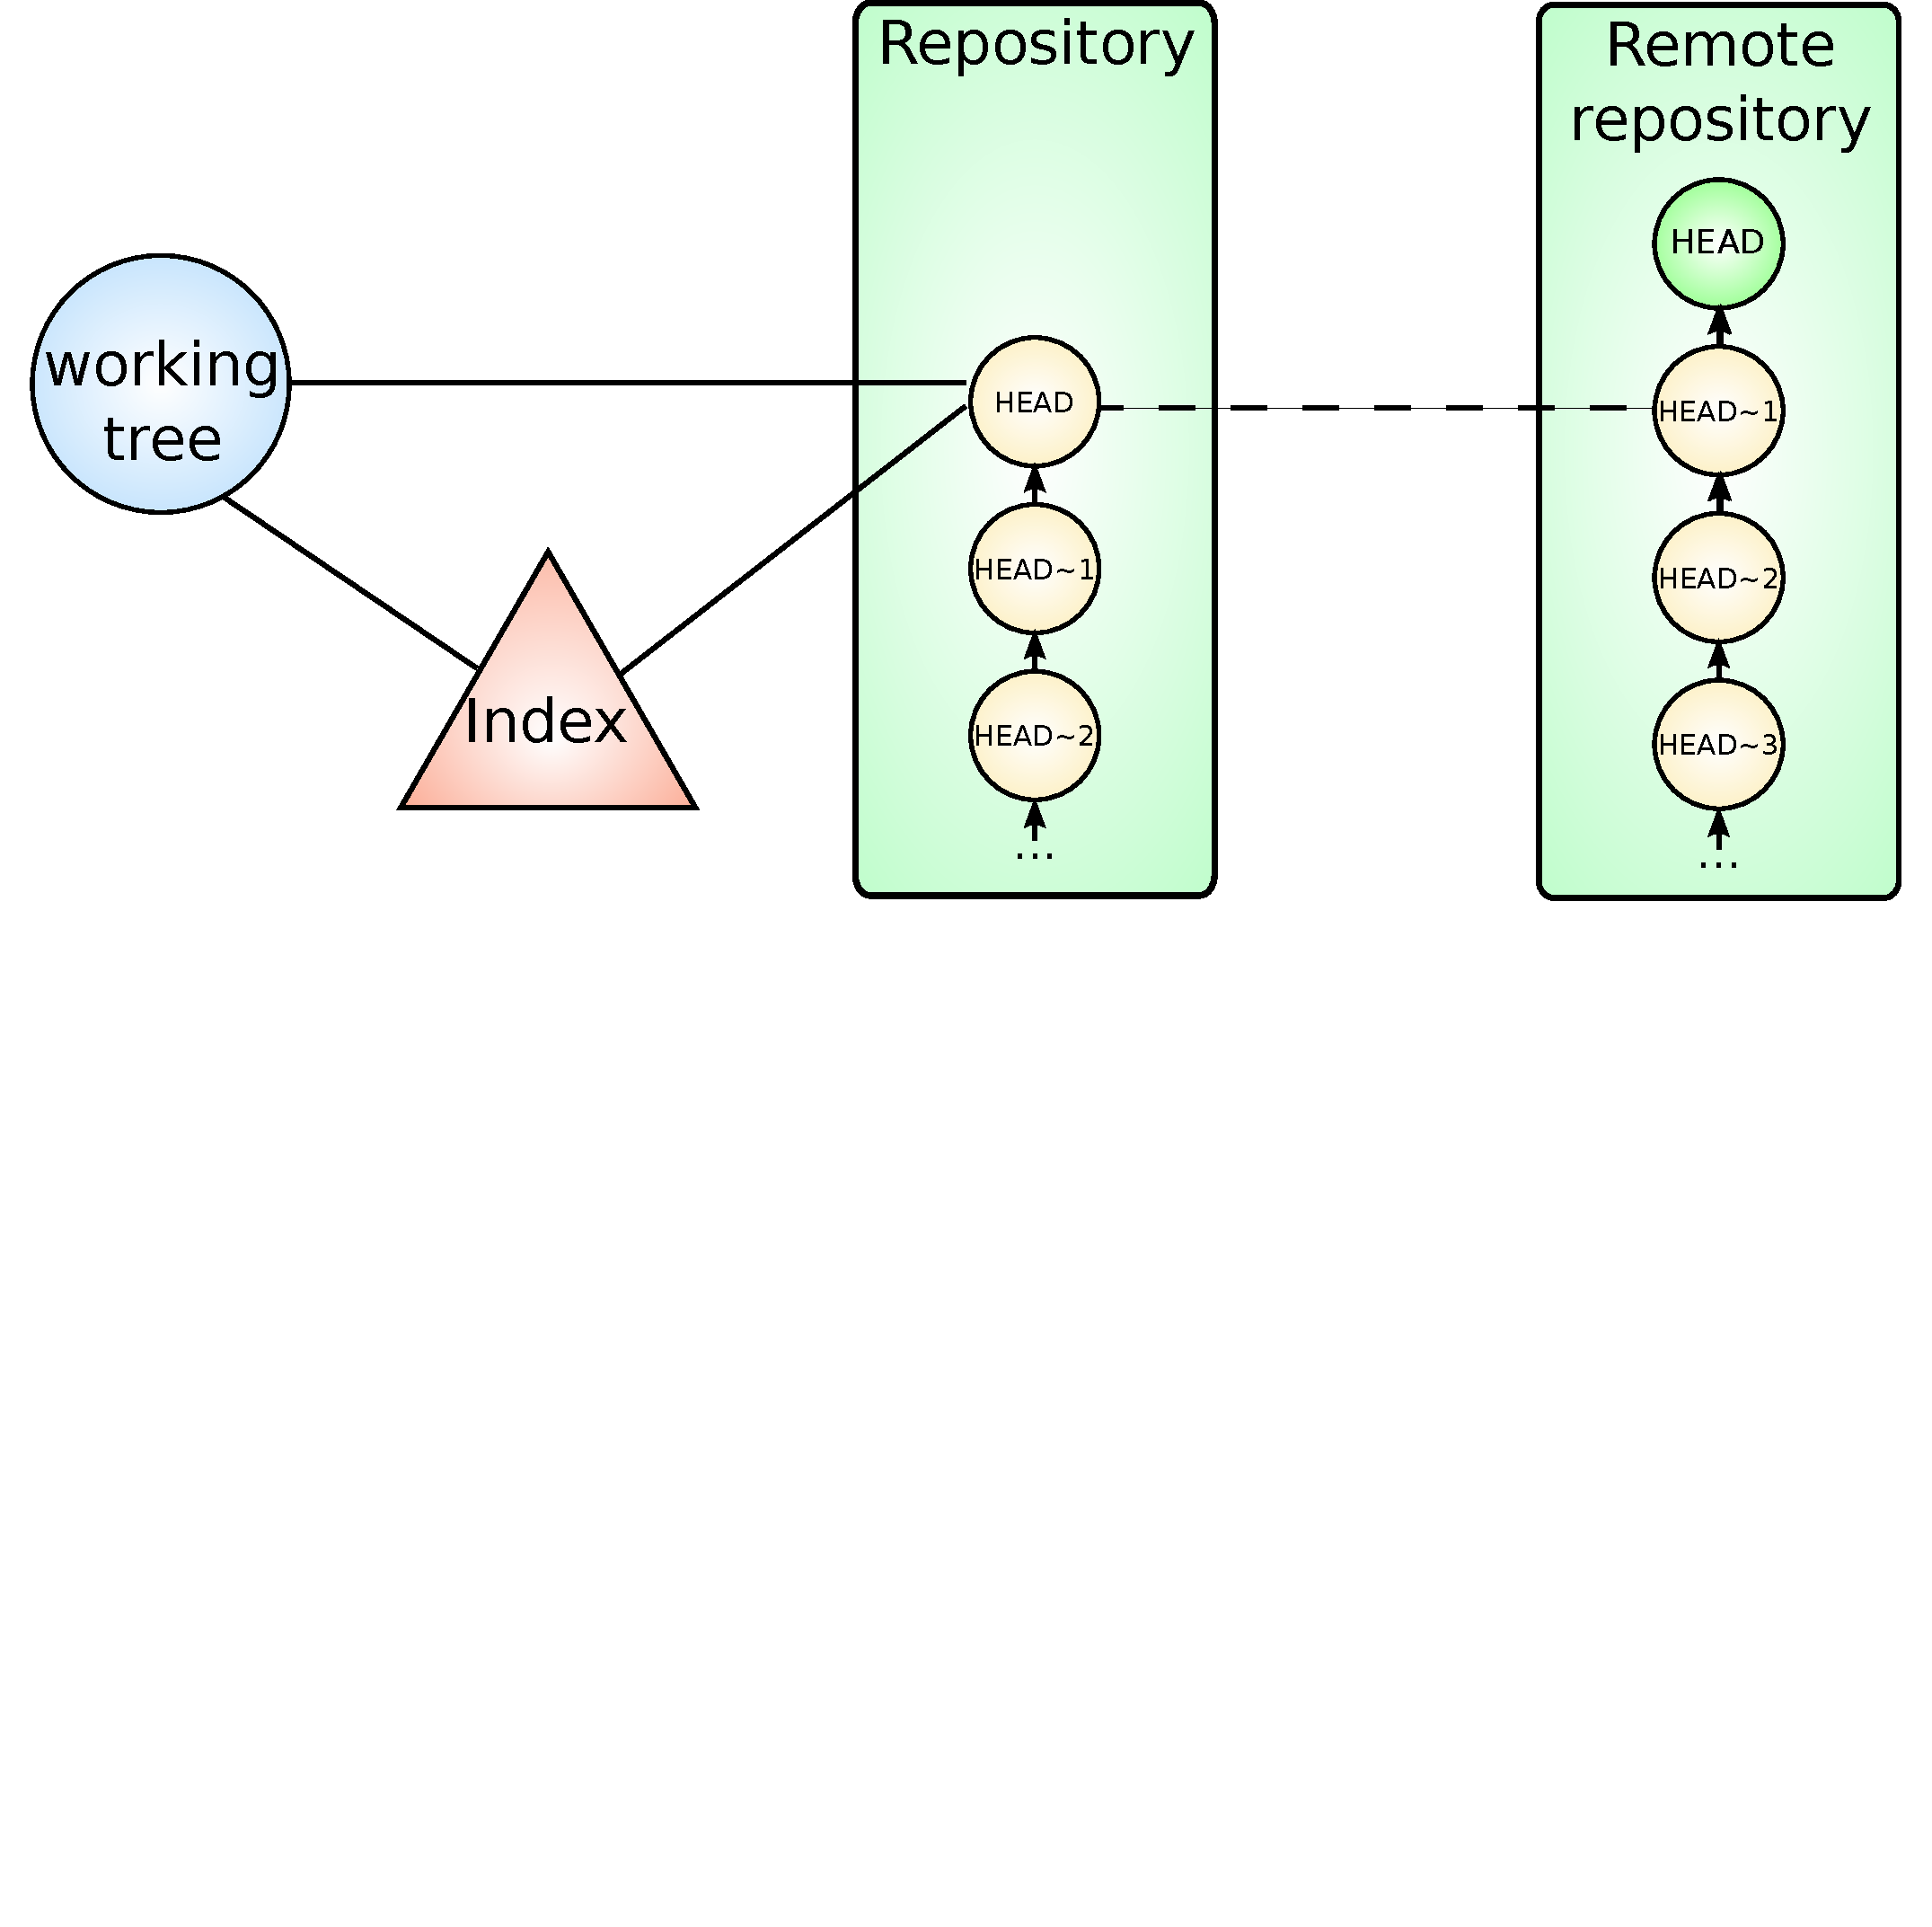
\includegraphics[height=0.8\textheight]{images/pdf/git-detailed-12.pdf}}
    \only<2>{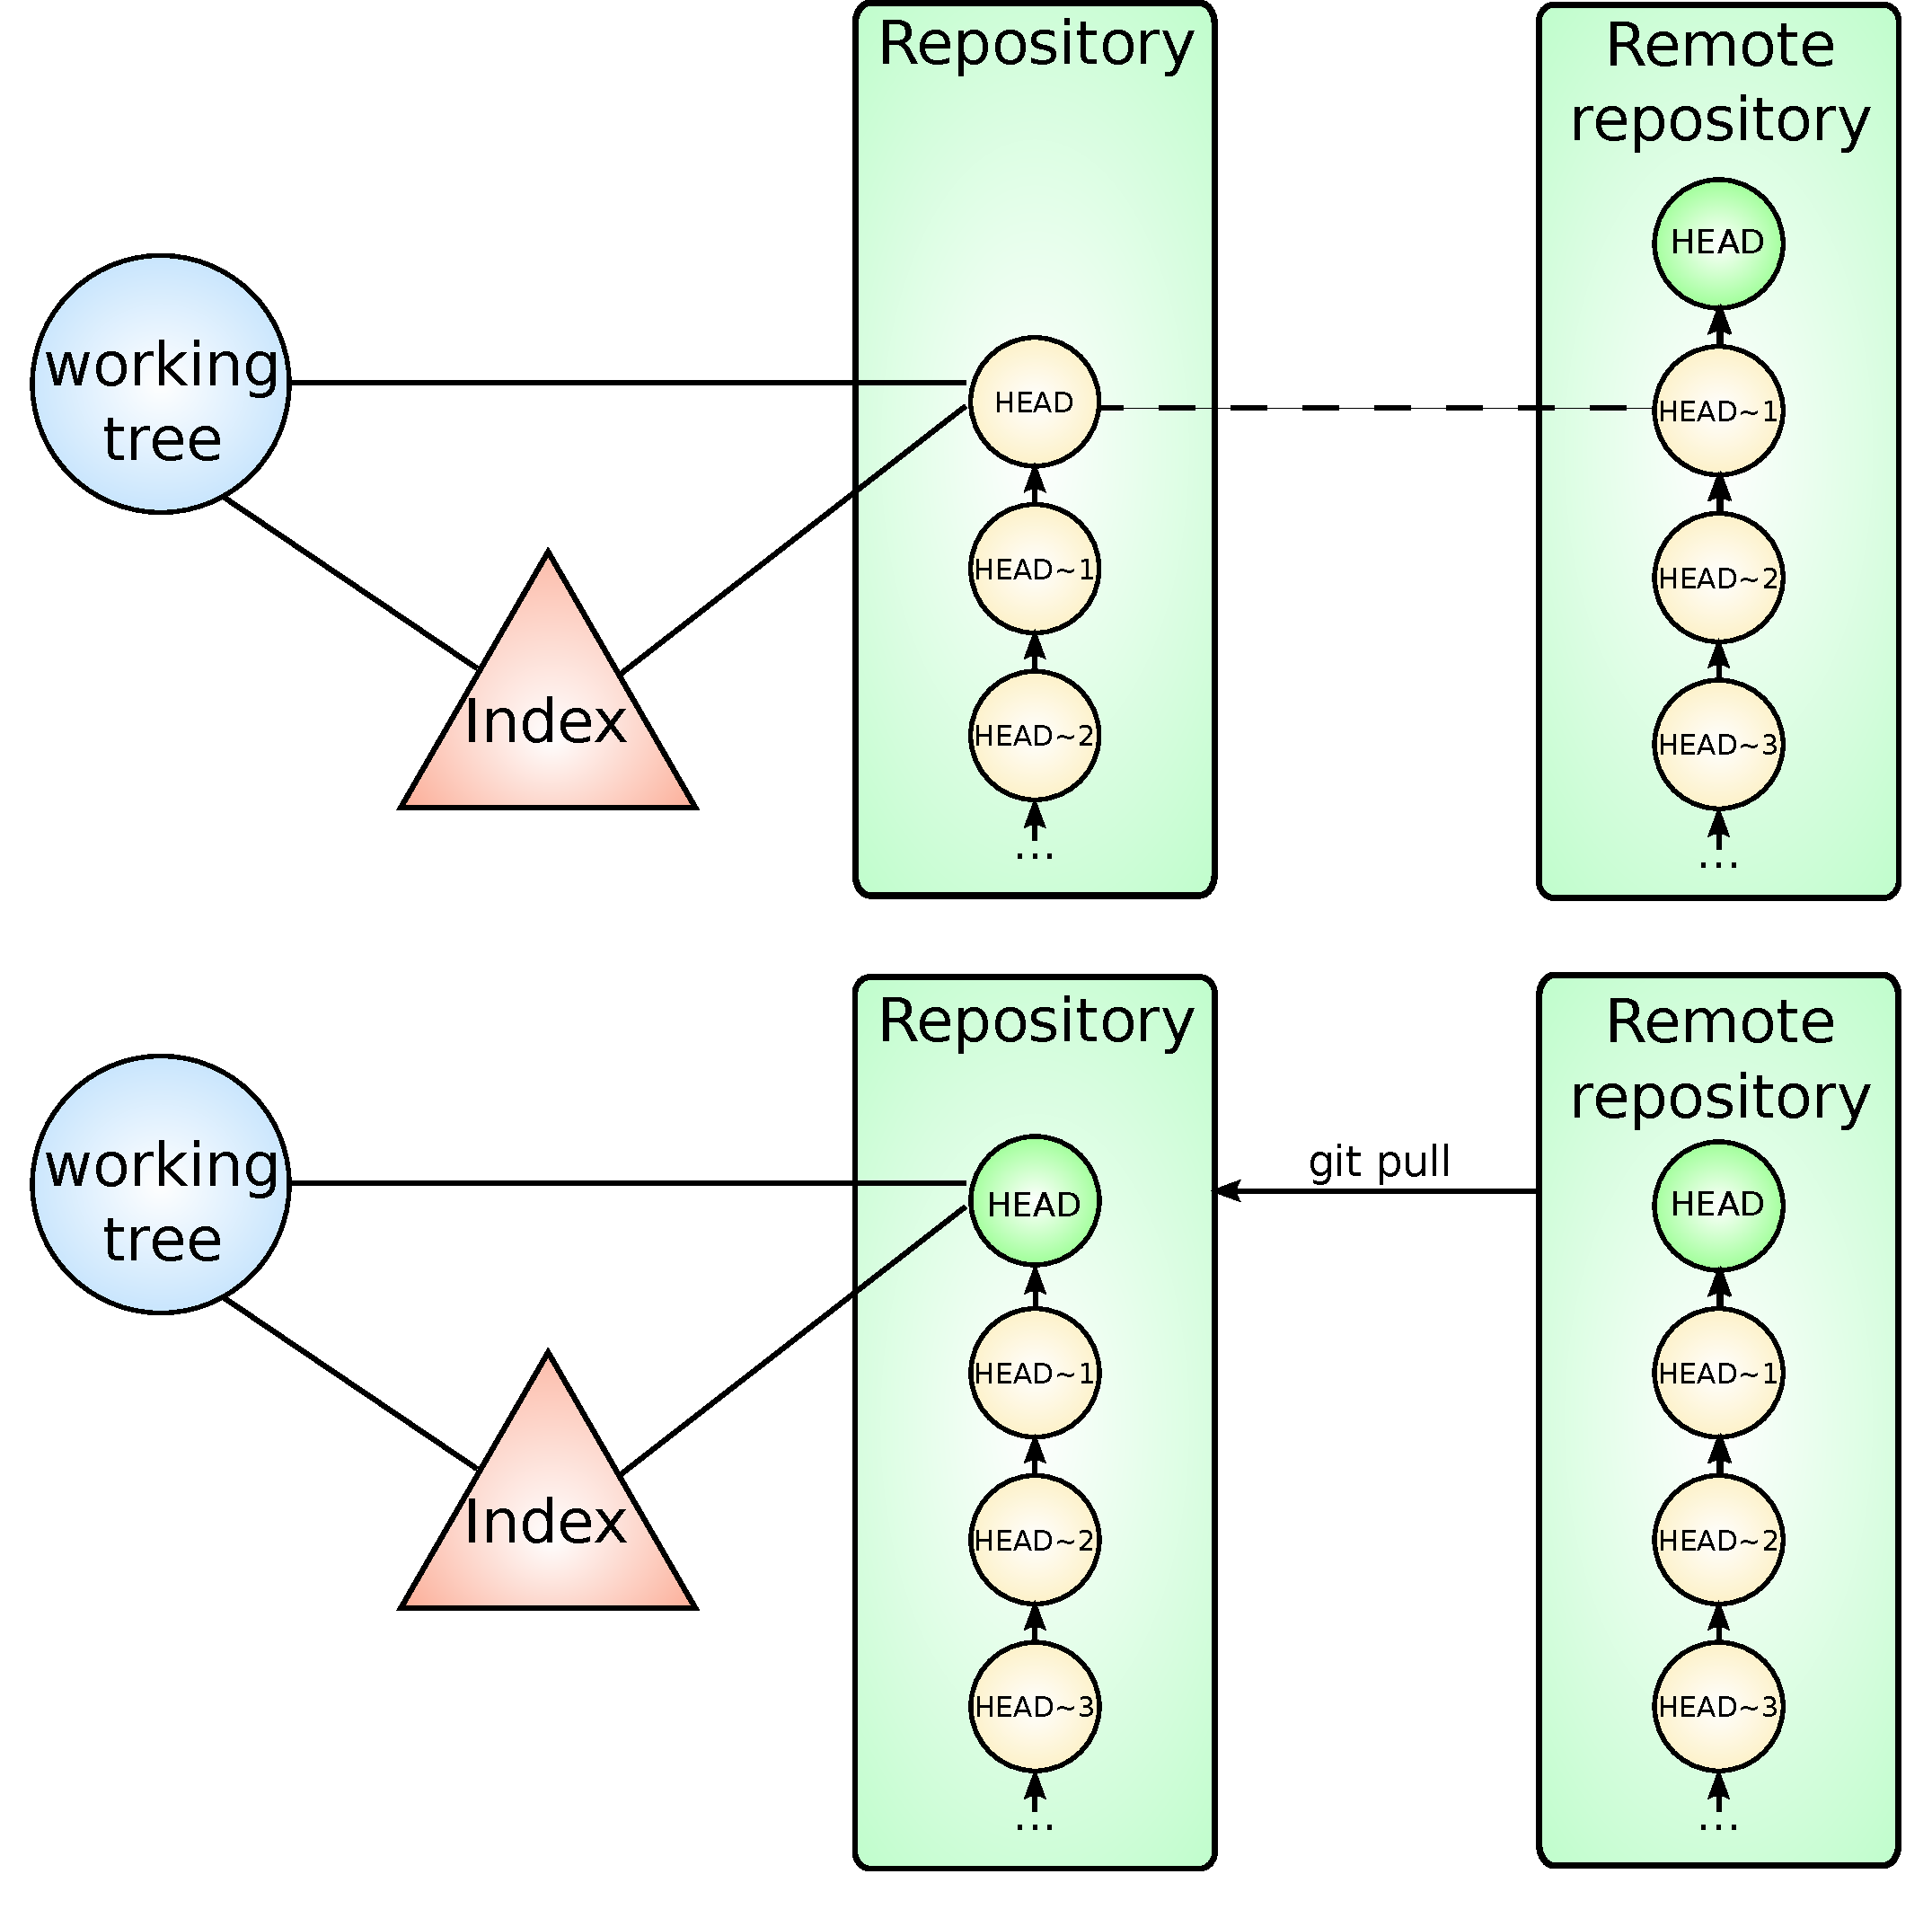
\includegraphics[height=0.8\textheight]{images/pdf/git-detailed-13.pdf}}
  \end{center}
\end{frame}

%%%%%%%%%%%%%%%%%%%%%%%%%%

\subsection{Typical workflow in git - an example}
\begin{frame}[fragile]
  \frametitle{\insertsubsection}

  \begin{small}
\begin{verbatim}
$ mkdir /tmp/git
$ cd /tmp/git

$ git init .                # Initialize repository
Initialized empty Git repository in /tmp/git/.git/

$ touch A B C
$ git add A B C             # Add new files to Index

$ git commit -m "Initial commit"  # First commit!
[master (root-commit) fa16ae4] Initial commit
 0 files changed, 0 insertions(+), 0 deletions(-)
 create mode 100644 A
 create mode 100644 B
 create mode 100644 C
\end{verbatim}
  \end{small}

\end{frame}
\begin{frame}[fragile]
  \frametitle{\insertsubsection}

  \begin{small}
\begin{verbatim}
$ git diff --stat           # Working Tree <-> Index
$ git diff --stat HEAD      # Working Tree <-> HEAD
$ git diff --stat --cached  # Index <-> HEAD

  <<< MAKE SOME CHANGES IN THE WORKING TREE >>>

$ git diff --stat           # Working Tree <-> Index
 A |    3 +++
 C |    3 +++
 2 files changed, 3 insertions(+), 0 deletions(-)

$ git diff --stat HEAD      # Working Tree <-> HEAD
 A |    3 +++
 C |    3 +++
 2 files changed, 3 insertions(+), 0 deletions(-)

$ git diff --stat --cached  # Index <-> HEAD
\end{verbatim}
  \end{small}

\end{frame}
\begin{frame}[fragile]
  \frametitle{\insertsubsection}

  \begin{small}
\begin{verbatim}
$ git add A C               # Move changes to Index

$ git diff --stat           # Working Tree <-> Index

$ git diff --stat HEAD      # Working Tree <-> HEAD
 A |    3 +++
 C |    3 +++
 2 files changed, 3 insertions(+), 0 deletions(-)

$ git diff --stat --cached  # Index <-> HEAD
 A |    3 +++
 C |    3 +++
 2 files changed, 3 insertions(+), 0 deletions(-)
\end{verbatim}
  \end{small}

\end{frame}
\begin{frame}[fragile]
  \frametitle{\insertsubsection}

  \begin{small}
\begin{verbatim}
$ git commit -m "My first patch :-)"   # Commit changes
[master 614c4e2] My first patch :-)
 2 files changed, 3 insertions(+), 0 deletions(-)

$ git diff --stat           # Working Tree <-> Index
$ git diff --stat HEAD      # Working Tree <-> HEAD
$ git diff --stat --cached  # Index <-> HEAD

$ git show --stat HEAD      # Show last commit's stats
commit 614c4e224284e2719fe040b64685b790606000a6
Author: Mario Sanchez Prada <mario@mariospr.org>
Date:   Mon May 3 09:31:19 2013 +0200

    My first patch :-)

 A |    3 +++
 C |    3 +++
 2 files changed, 3 insertions(+), 0 deletions(-)
\end{verbatim}
  \end{small}
\end{frame}
\begin{frame}[fragile]
  \frametitle{\insertsubsection}

  \begin{small}
\begin{verbatim}
$ git log                   # Show history up-to-date
commit 614c4e224284e2719fe040b64685b790606000a6
Author: Mario Sanchez Prada <mario@mariospr.org>
Date:   Mon May 3 09:31:19 2013 +0200

    My first patch :-)

commit fa16ae4ff64b3b968ca8991c90f123e62a6a009c
Author: Mario Sanchez Prada <mario@mariospr.org>
Date:   Mon May 3 09:30:11 2013 +0200

    Initial commit
\end{verbatim}
  \end{small}

\end{frame}

%%%%%%%%%%%%%%%%%%%%%%%%%%

\subsection{Typical workflow in git (wrapping up)}

\begin{frame}
  \frametitle{\insertsubsection}

  \textbf{Basic commands\only<2>{ (extended version)}:}
  \begin{itemize}

  \item \texttt{git init}: Initializes the repository to work with
    \git \vspacing

  \item \texttt{git add}: Adds changes in the \textit{Working Tree} to
    the\textit{Index}
    \only<2>{
    \begin{itemize}
    \item \texttt{git add -u}: Adds all the changes to the \textit{Index}
    \item \texttt{git add --patch}: Interactively asks which changes
      should go to the \textit{Index} (\textit{hunk} by \textit{hunk})
    \end{itemize}}
    \vspacing

  \item \texttt{git commit}: Makes changes in the \textit{Index}
    permanent, creating a new commit and updating the \textit{HEAD}.
    \only<2>{
    \begin{itemize}
    \item \texttt{git commit -a}: \texttt{git add -u \&\& git commit}
    \end{itemize}}
    \vspacing

  \item \texttt{git diff}: Differences between \textit{Working Tree} and
    \textit{Index}
    \only<2>{
    \begin{itemize}
    \item \texttt{git diff HEAD}: Diff between \textit{Working
        Tree} and \textit{HEAD}
    \item \texttt{git diff --cached}: Diff between \textit{Index} and \textit{HEAD}
    \end{itemize}}
    \vspacing

  \item \texttt{git push}: Sends local commits to a remote repository\vspacing

  \item \texttt{git pull}: Brings commits from a remote repository\vspacing

  \end{itemize}
\end{frame}

%%%%%%%%%%%%%%%%%%%%%%%%%%

\subsection{Typical workflow in git (wrapping up)}

\begin{frame}
  \frametitle{\insertsubsection}

  \textbf{Other (extremely useful) commands:}
  \begin{itemize}

  \item \texttt{git clone <URL>}: Clones a remote repository
    \vspacing

  \item \texttt{git rm <file>}: Removes \texttt{file} and get the
    \textit{Index} ready with the changes for the next
    \textit{commit}. \vspacing

  \item \texttt{git mv <fileA> <fileB>}: Renames \texttt{fileA} as
    \texttt{fileB } and get the \textit{Index} ready with the changes.  \vspacing

  \item \texttt{git log}: Shows the full (\textit{log}) from
    \textit{HEAD} \vspacing

  \item \texttt{git status}: Shows the status of \textit{Working
      Tree} and \textit{Index} \vspacing

  \item \texttt{git show <commitID>}: Visualizes \textit{commit}
    \texttt{commitID} \vspacing
  \end{itemize}
\end{frame}


\begin{frame}[fragile]
  \frametitle{\insertsubsection: git status}

  \begin{tiny}
\begin{verbatim}
<<< RIGHT BEFORE ADDING A AND C TO INDEX WITH 'git add A C' >>>

$ git status
# On branch master
# Changed but not updated:
#   (use "git add <file>..." to update what will be committed)
#   (use "git checkout -- <file>..." to discard changes in working directory)
#
#	modified:   A
#	modified:   C
#
no changes added to commit (use "git add" and/or "git commit -a")

$ git add A

$ git status
# On branch master
# Changes to be committed:
#   (use "git reset HEAD <file>..." to unstage)
#
#	modified:   A
#
# Changed but not updated:
#   (use "git add <file>..." to update what will be committed)
#   (use "git checkout -- <file>..." to discard changes in working directory)
#
#	modified:   C
#

\end{verbatim}
  \end{tiny}

\end{frame}

\begin{frame}[fragile]
  \frametitle{\insertsubsection: git show}

  \begin{tiny}
\begin{verbatim}
<<< RIGHT AFTER COMMITING CHANGES WITH 'git commit' >>>

$ git show
commit 614c4e224284e2719fe040b64685b790606000a6
Author: Mario Sanchez Prada <mario@mariospr.org>
Date:   Mon May 3 09:31:19 2013 +0200

    My first patch :-)

diff --git a/A b/A
index e69de29..1802a74 100644
--- a/A
+++ b/A
@@ -0,0 +1,3 @@
+aaa
+bbb
+ccc
diff --git a/C b/C
index e69de29..1802a74 100644
--- a/C
+++ b/C
@@ -0,0 +1,3 @@
+aaa
+bbb
+ccc
\end{verbatim}
  \end{tiny}

\end{frame}

%%%%%%%%%%%%%%%%%%%%%%%%%%

\subsection{Comparing commands: Subversion - Git}

\begin{frame}
  \frametitle{\insertsubsection}

  \begin{center}
    \begin{tabular}{|c|c|}
      \hline \textbf{Subversion} & \textbf{Git} \\
      \hline \texttt{svnadmin create \textit{repo}} & \texttt{git init} \\
             \texttt{svn import \textit{filepath}} & \texttt{git add \textit{filepath}} \\
             \ & \texttt{git commit} \\
      \hline \texttt{svn checkout \textit{URL}} & \texttt{git clone
        \textit{URL}} \\
      \hline \texttt{svn add|rm|mv \textit{file}} & \texttt{git
        add|rm|mv \textit{file}} \\
      \hline \texttt{svn diff} & \texttt{git diff} \\
      \hline \texttt{svn commit} & \texttt{git commit -a} \\
             \ & \texttt{git push} \\
      \hline \texttt{svn update} & \texttt{git pull} \\
      \hline \texttt{svn status} & \texttt{git status} \\
      \hline \texttt{svn log} & \texttt{git log} \\
      \hline \texttt{svn blame \textit{file}} & \texttt{git blame
        \textit{file}} \\
      \hline
    \end{tabular}
  \end{center}
\end{frame}

%%%%%%%%%%%%%%%%%%%%%%%%%%

\section{Repositories and branches}

\subsection{Repositories}

\begin{frame}
  \frametitle{\insertsubsection}

  \textbf{Two types} of repositories: \vspacing
  \begin{itemize}
  \item \textbf{Local repository}: Local working directory under
    version control with \git (it contains a \texttt{.git/}
    directory)\\ \vspacing They can be ``created'' by either:\vspacing
    \begin{itemize}
    \item \texttt{git init}: Initializes the current directory to be
      used with \git (needed to \texttt{git add <file>} and
      \texttt{git commit}) \vspacing

    \item \texttt{git clone <URL>}: Clones a remote repository in a
      local directory, stablishing a link to the original one,
      throughout the remote repository \texttt{origin}.
    \end{itemize} \vspacing

  \item \textbf{Remote repositories}: Any non-local repository where
    we have cloned our local working directory from\\
    \vspacing

    Can be linked with \texttt{git remote add <name> <URL>} \\
    \texttt{git clone <URL>} automatically creates one: \texttt{origin}
  \end{itemize}\
\end{frame}

%%%%%%%%%%%%%%%%%%%%%%%%%%

\subsection{What's a branch?}

\begin{frame}
  \frametitle{\insertsubsection}

  A \textit{branch} is a paralell line of work which allow us to make
  and try out certain changes from a given point on, without altering
  the original line of work it was created from.\pause
  \\ \ \vspacing

  Once the changes done in the \textit{branch} have been proved to
  work well, they can be integrated in the original \textit{branch},
  resolving the ``conflicts'' that could have appeared since its
  creation.\pause \\ \ \vspacing

  Implementation:
  \begin{itemize}
  \item \textbf{In other \textit{VCS's} (\textit{Subversion})}: Separate directories \vspacing

  \item \textbf{En \git}: An \textit{alias} to the \textit{commit}
    that will be the \textit{HEAD} for that \textit{branch}
    (almost-zero cost, really fast).
  \end{itemize}
\end{frame}

%%%%%%%%%%%%%%%%%%%%%%%%%%

\subsection{What's a branch? - Subversion vs Git}

\begin{frame}
  \frametitle{\insertsubsection}

  \begin{center}
    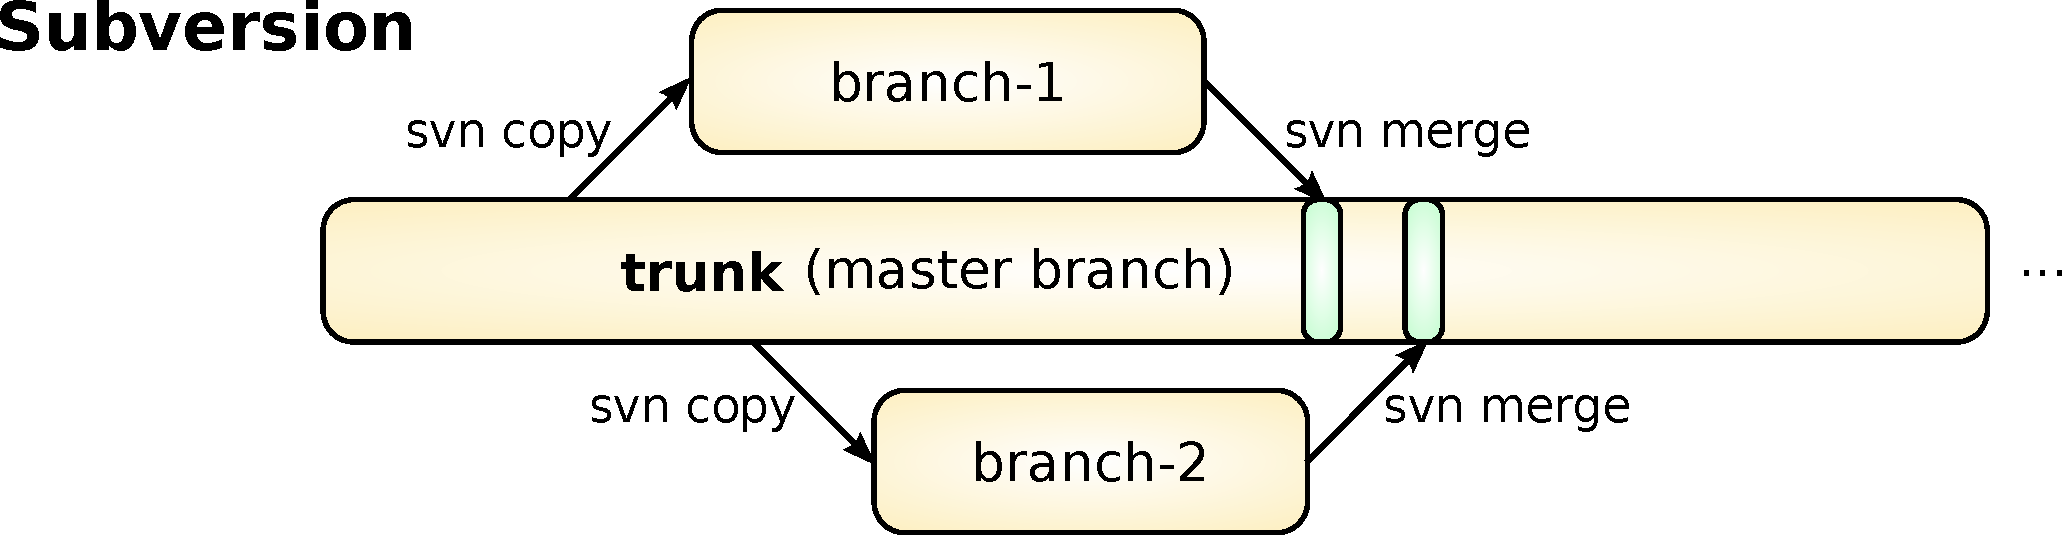
\includegraphics[width=1.0\textwidth]{images/pdf/svn-branches.pdf}
  \end{center}

  \begin{center}
    \uncover<2->{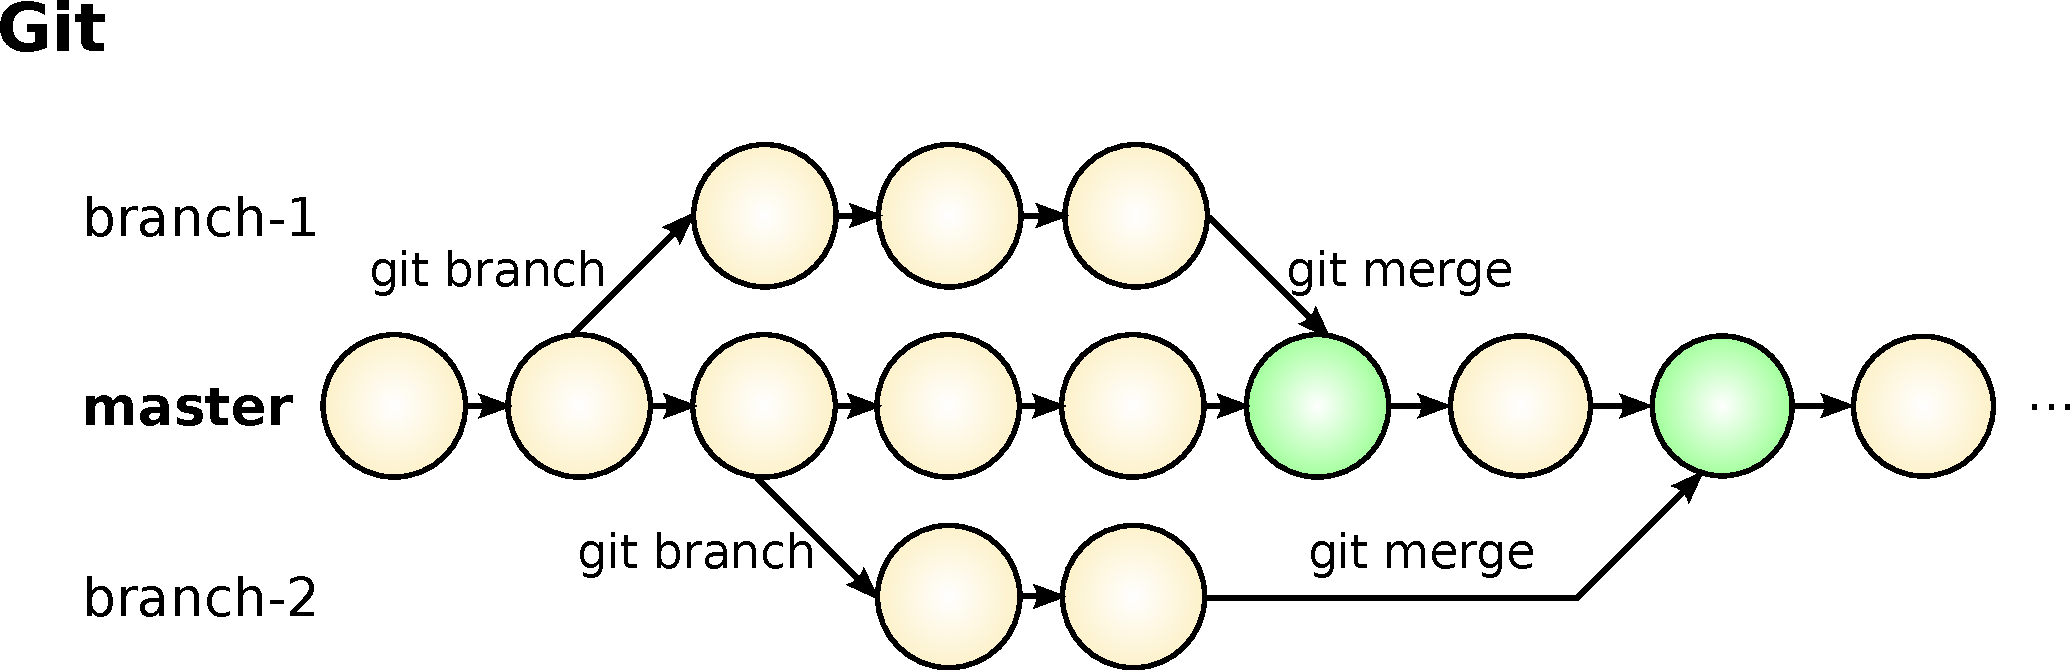
\includegraphics[width=1.0\textwidth]{images/pdf/git-branches.pdf}}
  \end{center}
\end{frame}

%%%%%%%%%%%%%%%%%%%%%%%%%%

\subsection{Branches in git}

\begin{frame}
  \frametitle{\insertsubsection}

  \begin{itemize}
  \item Create a new branch:\\
    \texttt{git branch <branch-name> [<start-point>]}
    \vspacing
  \item Delete a branch:\\
    \texttt{git branch (-d | -D) <branch-name>}
    \vspacing
  \item Rename a branch:\\
    \texttt{git branch -m <old-name> <new-name>}
    \vspacing
  \item List the current branches:\\
    \texttt{git branch [ -r | -a ]}
    \vspacing
  \item ``Move'' into a branch (check it out):\\
    \texttt{git checkout [-b] <branch-name>}
    \vspacing
\end{itemize}
\end{frame}

\subsection{Branches in git - an example}
\begin{frame}[fragile]
  \frametitle{\insertsubsection}

  \begin{small}
\begin{verbatim}
$ git branch
* master

$ git branch mybranch-1

$ git branch mybranch-2

$ git branch
* master
  mybranch-1
  mybranch-2

$ git checkout mybranch-1
Switched to branch 'mybranch-1'

$ git branch
  master
* mybranch-1
  mybranch-2
\end{verbatim}
  \end{small}

\end{frame}
\begin{frame}[fragile]
  \frametitle{\insertsubsection}

  \begin{small}
\begin{verbatim}
$ git branch -m mybranch-1 branch-1
$ git branch -m mybranch-2 branch-2

$ git branch
  master
* branch-1
  branch-2

$ git checkout master
Switched to branch 'master'

$ git branch -d branch-1
Deleted branch branch-1 (was 59f1309).

$ git branch -d branch-2
Deleted branch branch-2 (was e721bce).

$ git branch
* master
\end{verbatim}
  \end{small}

\end{frame}

%%%%%%%%%%%%%%%%%%%%%%%%%%

\subsection{Why to use branches?}

\begin{frame}
  \frametitle{\insertsubsection}

  \begin{itemize}
  \item They are fast, convenient, and really ``cheap''\vspacing
  \item To try an idea out (experiment) \vspacing
  \item Separate public and private work \vspacing
  \item One branch per \textit{bug}/\textit{feature} \vspacing
  \item Prepare for a new \textit{release} (integration) \vspacing
  \item As a temporary \textit{backup} (\textit{snapshot}) \vspacing
  \item \textbf{It's the usual way of working with \git} \vspacing
  \end{itemize}
\end{frame}

%%%%%%%%%%%%%%%%%%%%%%%%%%

\subsection{Local branches and remote branches}

\begin{frame}
  \frametitle{\insertsubsection}

  \textbf{Two types} of branches:
  \begin{itemize}
  \item \textbf{Local branches}: Branches created in the local machine
    to work on top of them, making all the needed changes.\vspacing

  \item \textbf{Remote branches}: Branches from a remote repository
    that we can link to local branches to work with them.
  \end{itemize}\  \\ \ \\


  \textbf{Clarifications}:\\
  Both the \textbf{local} and the  \textbf{remote} branches are always
  in our \textbf{local repository} (local/remote concept depends on
  the POV). \vspacing

  The \textbf{remote} branches act as a \textit{cache} of non-local
  branches in \textbf{remote repositories} (they are \textit{rsync-ed}). \vspacing

  The \textbf{local} branches are \textit{pushed}/\textit{pulled} to/from the \textbf{remote
    repositories} throughout their associated \textbf{remote} branches.

\end{frame}

\subsection{Local branches and remote branches - an example}
\begin{frame}[fragile]
  \frametitle{\insertsubsection}

  \begin{small}
\begin{verbatim}
$ git branch -a
* master
  remotes/origin/master
  remotes/origin/other-branch

$ git branch private

$ git branch other-branch origin/other-branch
Branch other-branch set up to track
remote branch other-branch from origin.

$ git branch -a
* master
  private
  other-branch
  remotes/origin/master
  remotes/origin/other-branch
\end{verbatim}
  \end{small}

\end{frame}

%%%%%%%%%%%%%%%%%%%%%%%%%%

\subsection{An example of repositories and branches: epiphany}

\begin{frame}[fragile]
  \frametitle{\insertsubsection}

  \begin{columns}[t]
    \column{.6\textwidth}
    \begin{block}{Local branches}
      \begin{tiny}
\begin{verbatim}
$ git branch
  136292
  539716
  602547
  608980
* 611400
  alex
  master
\end{verbatim}
\end{tiny}
    \end{block} \vspacing
    Using branches in this example:
    \begin{itemize}
    \item One branch per \textit{bug} \vspacing

    \item One experimental branch (\texttt{alex}) \vspacing

    \item One ``main'' branch (\texttt{master}).
    \end{itemize}

    \column{.4\textwidth}
    \begin{block}{Remote branches}
      \begin{tiny}
\begin{verbatim}
$ git remote 
origin

$ git branch -r
  origin/HEAD -> origin/master
  origin/Release043
  origin/bookmarks-toolbars-changes
  origin/bookmarksbar-separation
  origin/css-fonts-branch
  origin/eog-menu-api
  origin/gnome-2-10
  [...]
  origin/master
  origin/mozilla-embed-strings
  origin/new-completion
  origin/new-downloader
  origin/pre-gnome-2-10
  origin/pre-gnome-2-14
  origin/pre-gnome-2-6
  origin/pre-gnome-2-8
  origin/release-1-2-1
  origin/webcore-branch
  origin/webkit
  origin/xulrunner
\end{verbatim}
\end{tiny}
    \end{block}
\end{columns}
\end{frame}

%%%%%%%%%%%%%%%%%%%%%%%%%%

\subsection{Updating the branches}

\begin{frame}
  \frametitle{\insertsubsection}

  \ \vspacing
  \textbf{Two typical situations}: \vspacing \ \vspacing
  \begin{itemize}

  \item \textbf{Add} changes in a \textbf{private branch} to a
    \textbf{public branch} (integrate local changes)
    \uncover<2->{
    \begin{itemize}
    \item We can't alter past history in a public branch
    \item We need ``clean'' changes ready to be applied on top of
      \textit{HEAD} in the public branch
    \end{itemize}}
    \vspacing

  \item \textbf{Modify} a \textbf{private branch} with new code from a
    \textbf{public branch} where it was created from (update)
    \uncover<3>{
    \begin{itemize}
    \item We can alter past history in a private branch
    \item It's more interesting to ``change the past'' whenever it's
      needed in order to always have ``clean changes'' in the branch
      where it was created from (it could have changed)
    \end{itemize}}

  \end{itemize}
\end{frame}

%%%%%%%%%%%%%%%%%%%%%%%%%%

\subsection{Updating branches - git merge}

\begin{frame}[fragile]
  \frametitle{\insertsubsection}

  \ \vspacing
  \textbf{Updating} a \textbf{public branch}: \texttt{git merge <branch>}
  \vspacing
  \begin{itemize}
    \begin{small}
  \item There are \textbf{no changes} in the public branch where the
    private one was created from:

  \begin{center}
    \only<2>{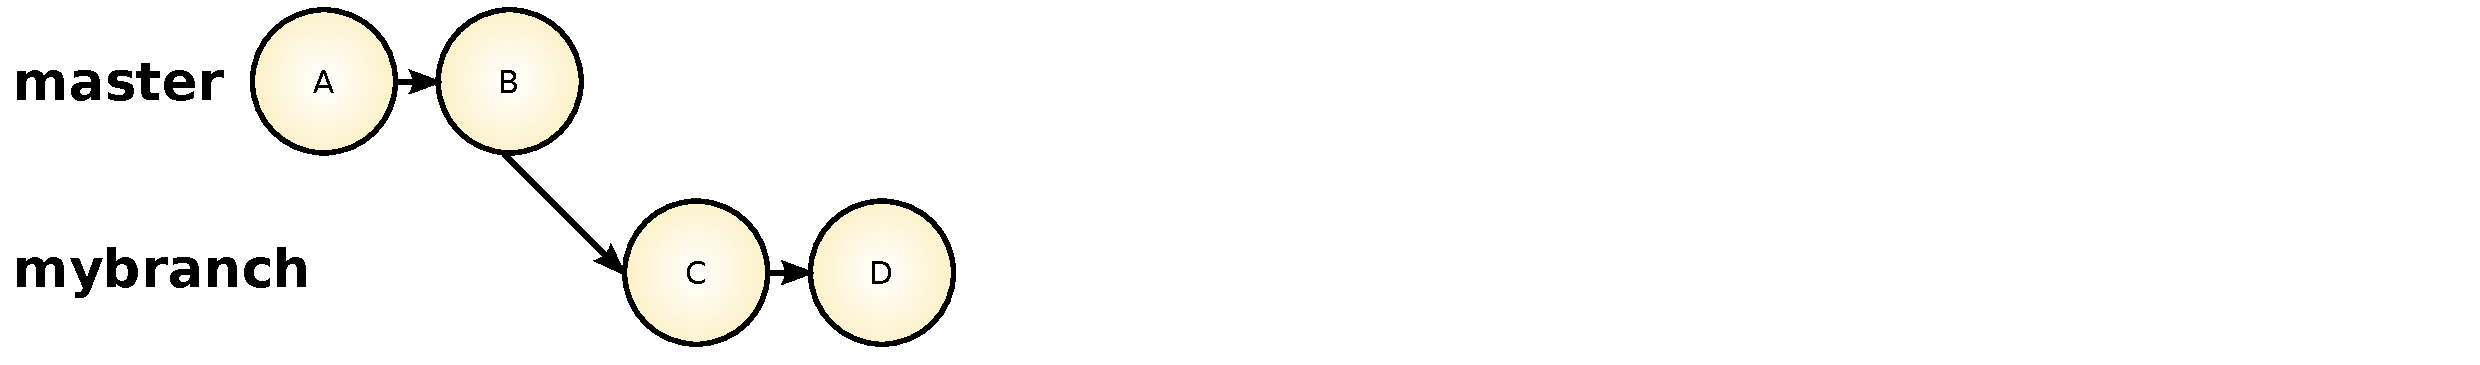
\includegraphics[width=1.00\textwidth]{images/pdf/git-merge-A1.pdf}}
    \only<3>{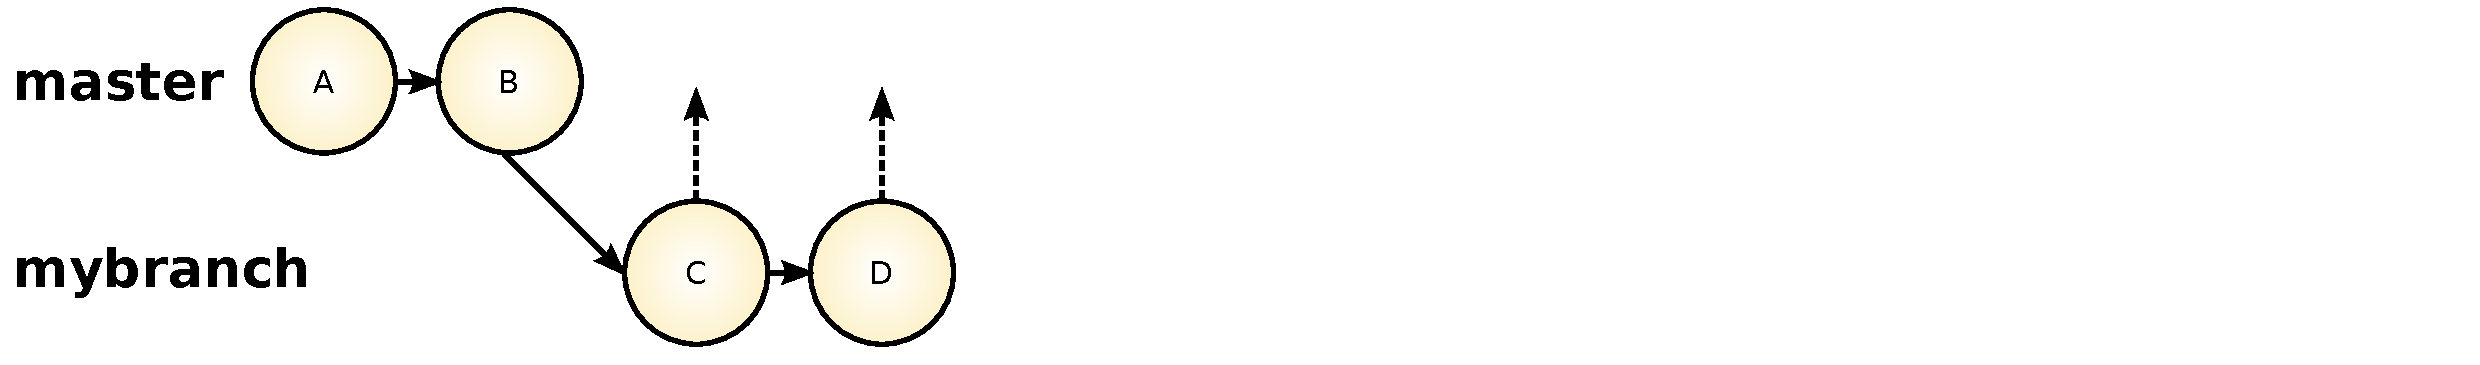
\includegraphics[width=1.00\textwidth]{images/pdf/git-merge-A2.pdf}}
    \only<4->{
\includegraphics[width=1.00\textwidth]{images/pdf/git-merge-A3.pdf}}
  \end{center}

  \item There are \textbf{changes} in the public branch where the
    private one was created from:

    \begin{center}
      \only<5>{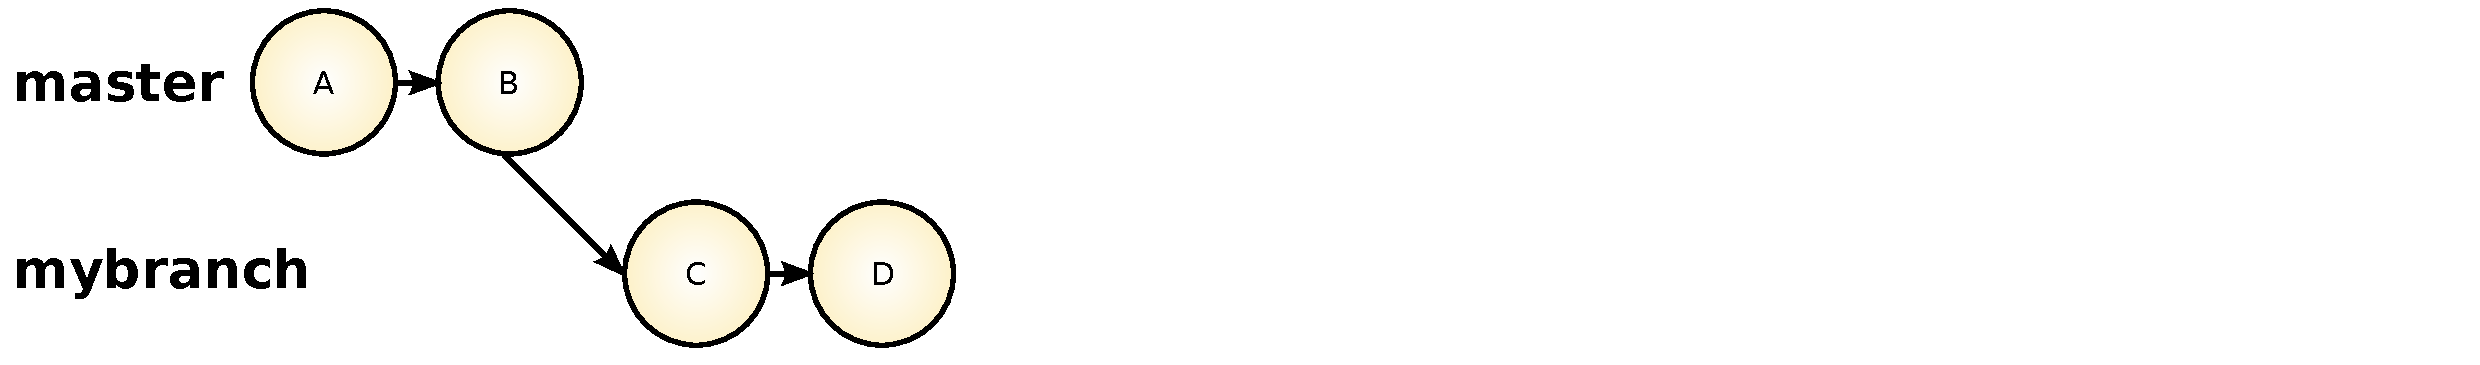
\includegraphics[width=1.00\textwidth]{images/pdf/git-merge-B1.pdf}}
      \only<6>{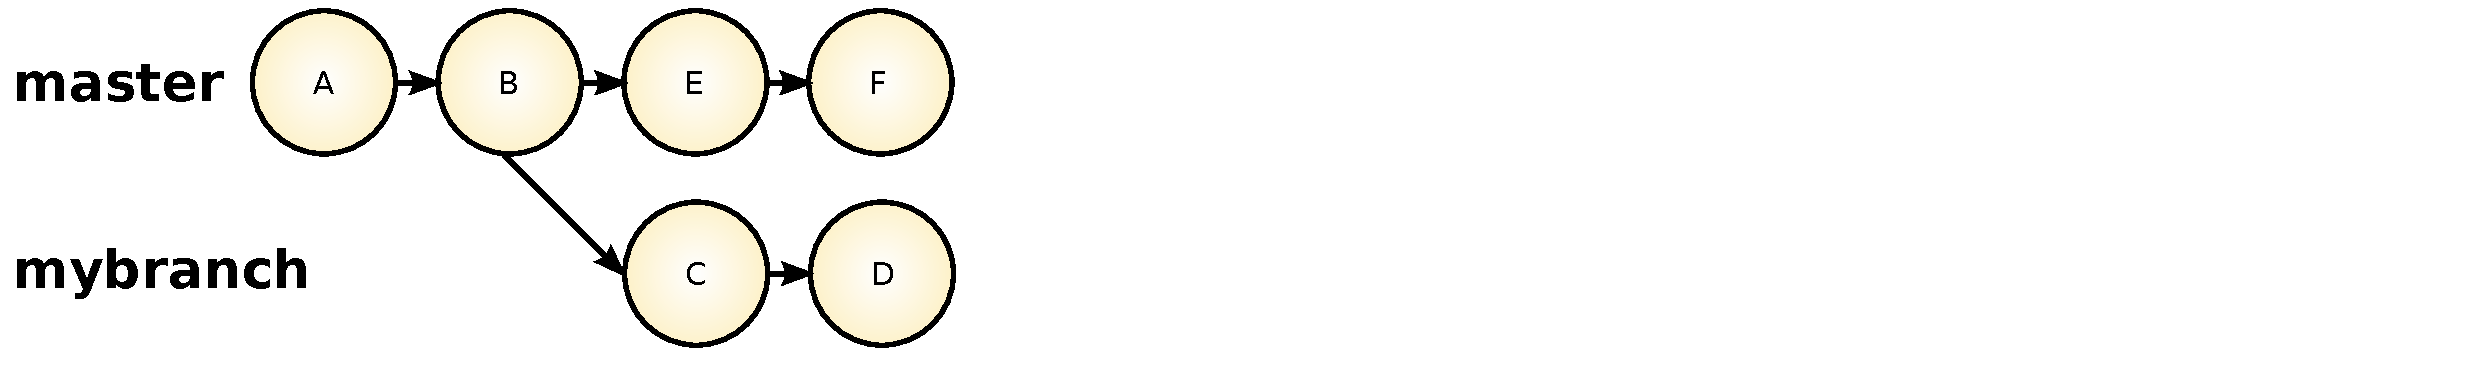
\includegraphics[width=1.00\textwidth]{images/pdf/git-merge-B2.pdf}}
      \only<7>{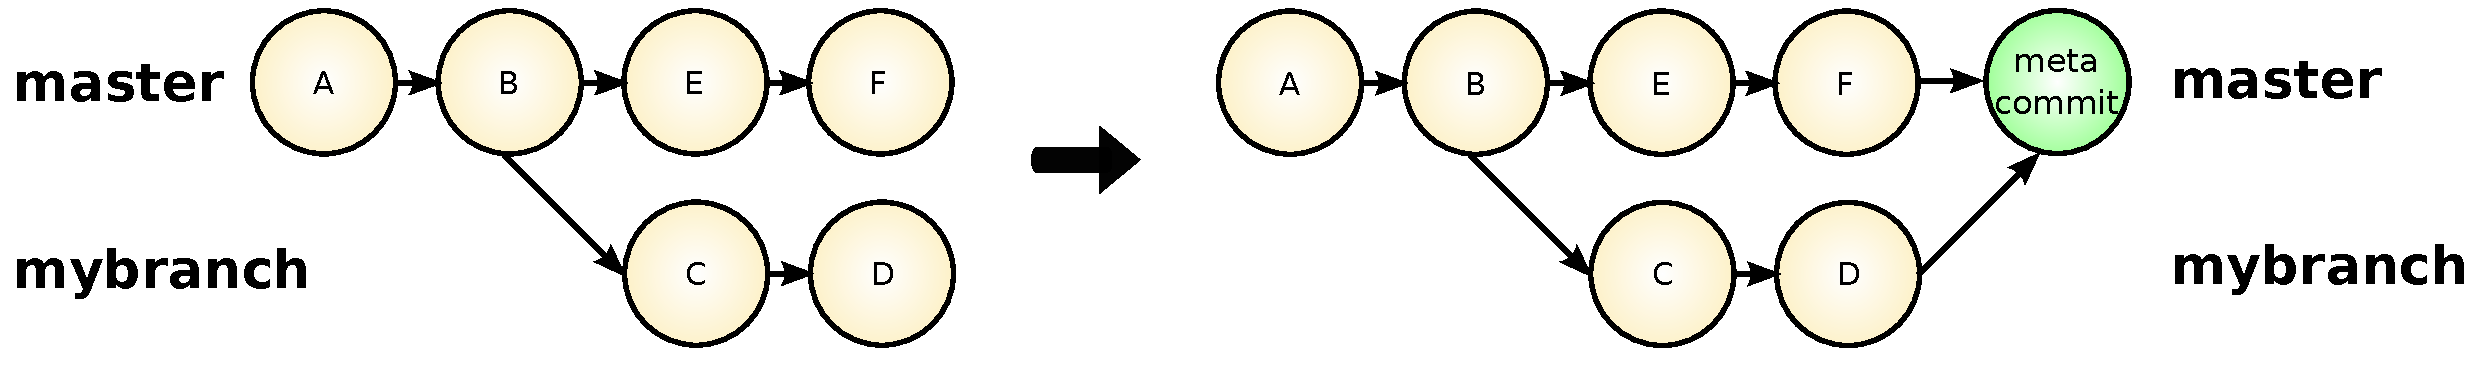
\includegraphics[width=1.00\textwidth]{images/pdf/git-merge-B3.pdf}}
    \end{center}

    \end{small}
  \end{itemize}
\end{frame}

%%%%%%%%%%%%%%%%%%%%%%%%%%

\subsection{Updating branches - git rebase}

\begin{frame}[fragile]
  \frametitle{\insertsubsection}

  \ \vspacing
  \textbf{Update} a \textbf{private branch}:  \texttt{git rebase <new-base>}
  \vspacing
  \begin{center}
    \only<1>{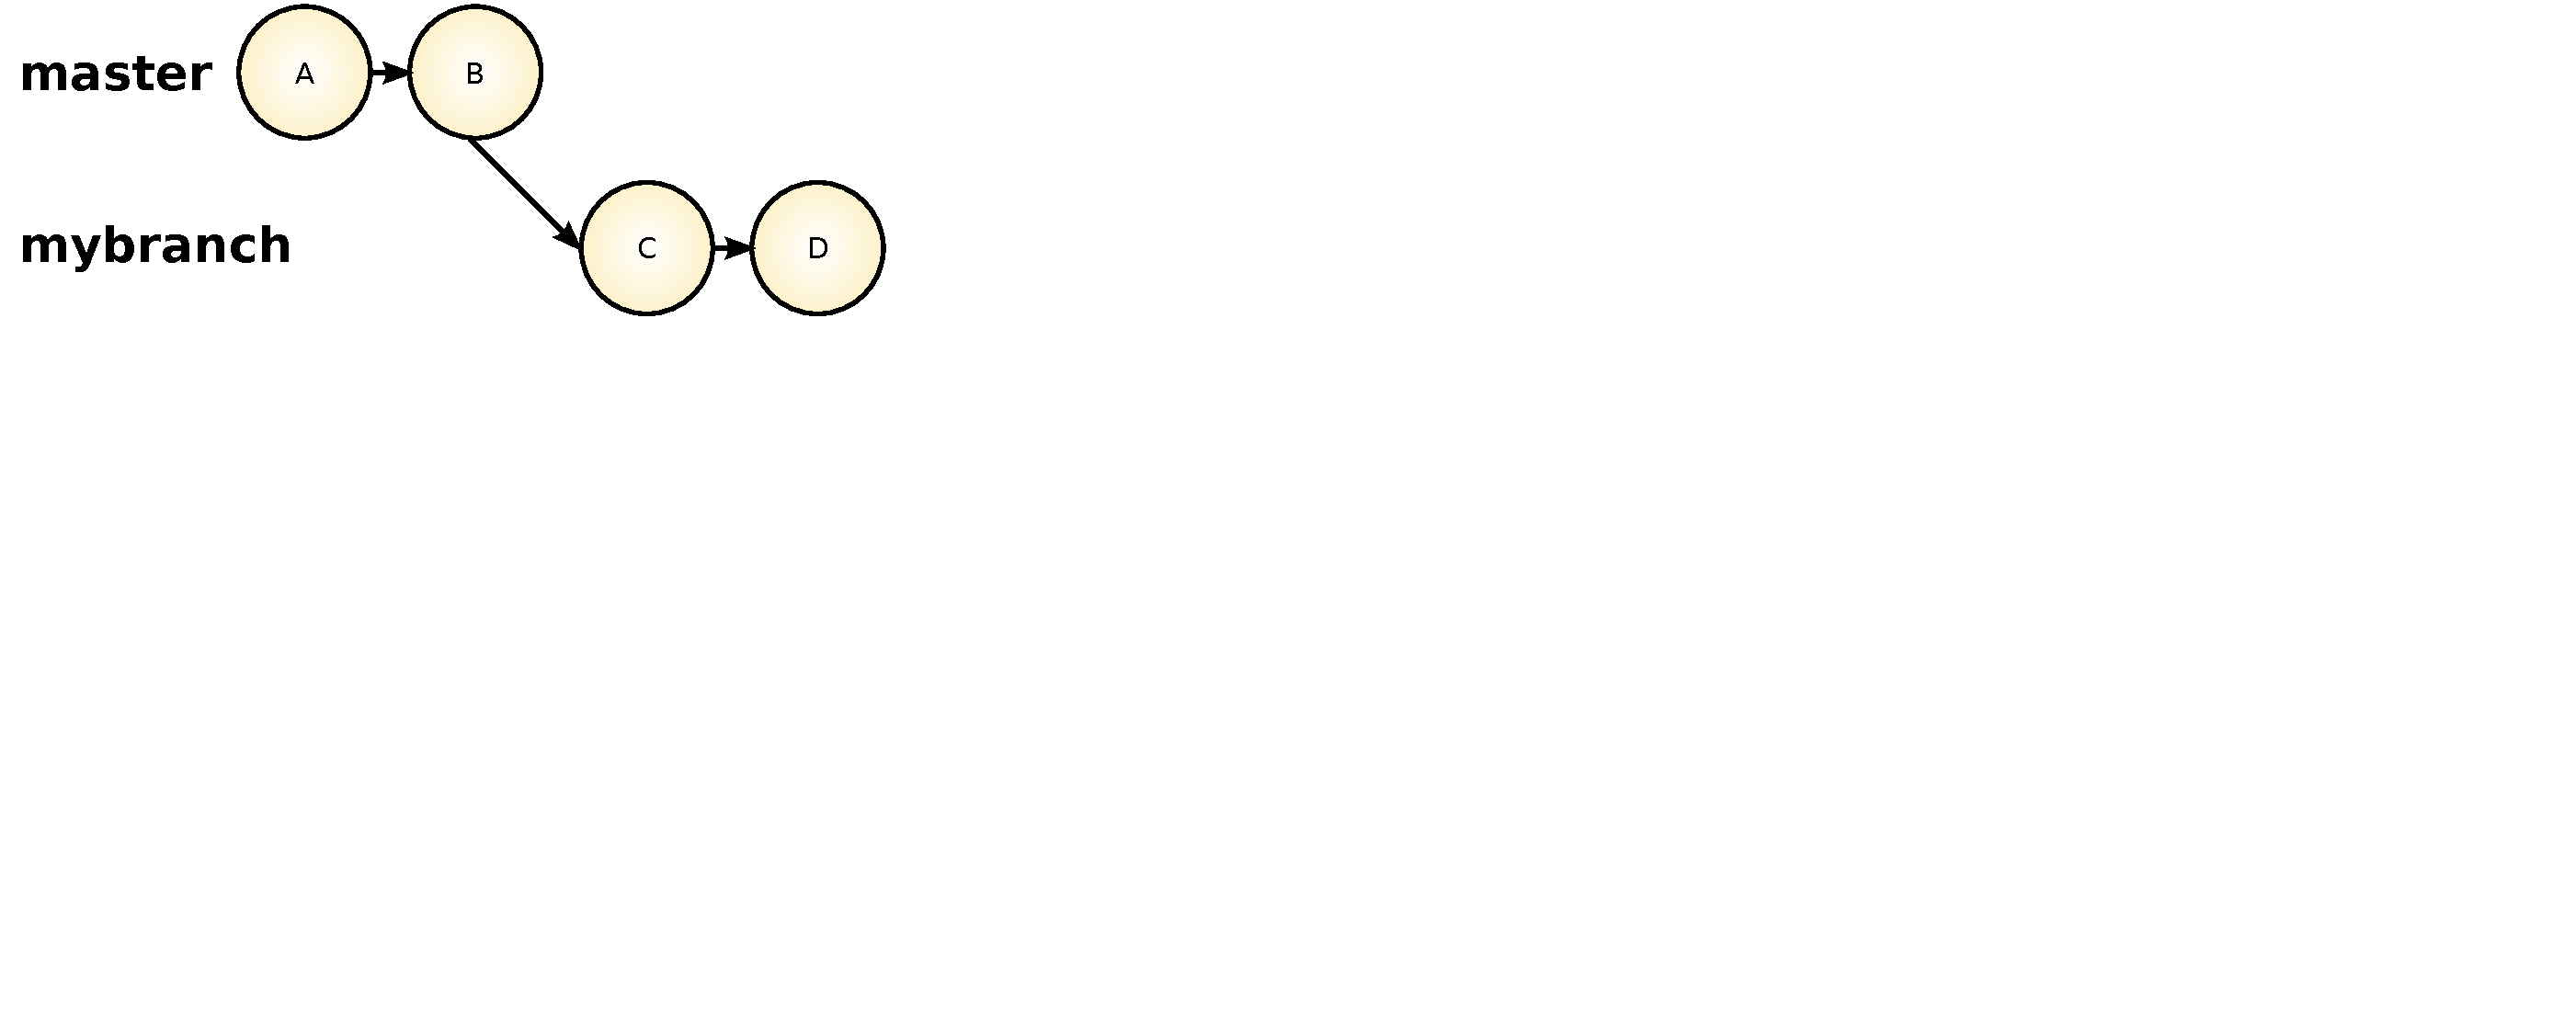
\includegraphics[width=1.00\textwidth]{images/pdf/git-rebase-0.pdf}}
    \only<2>{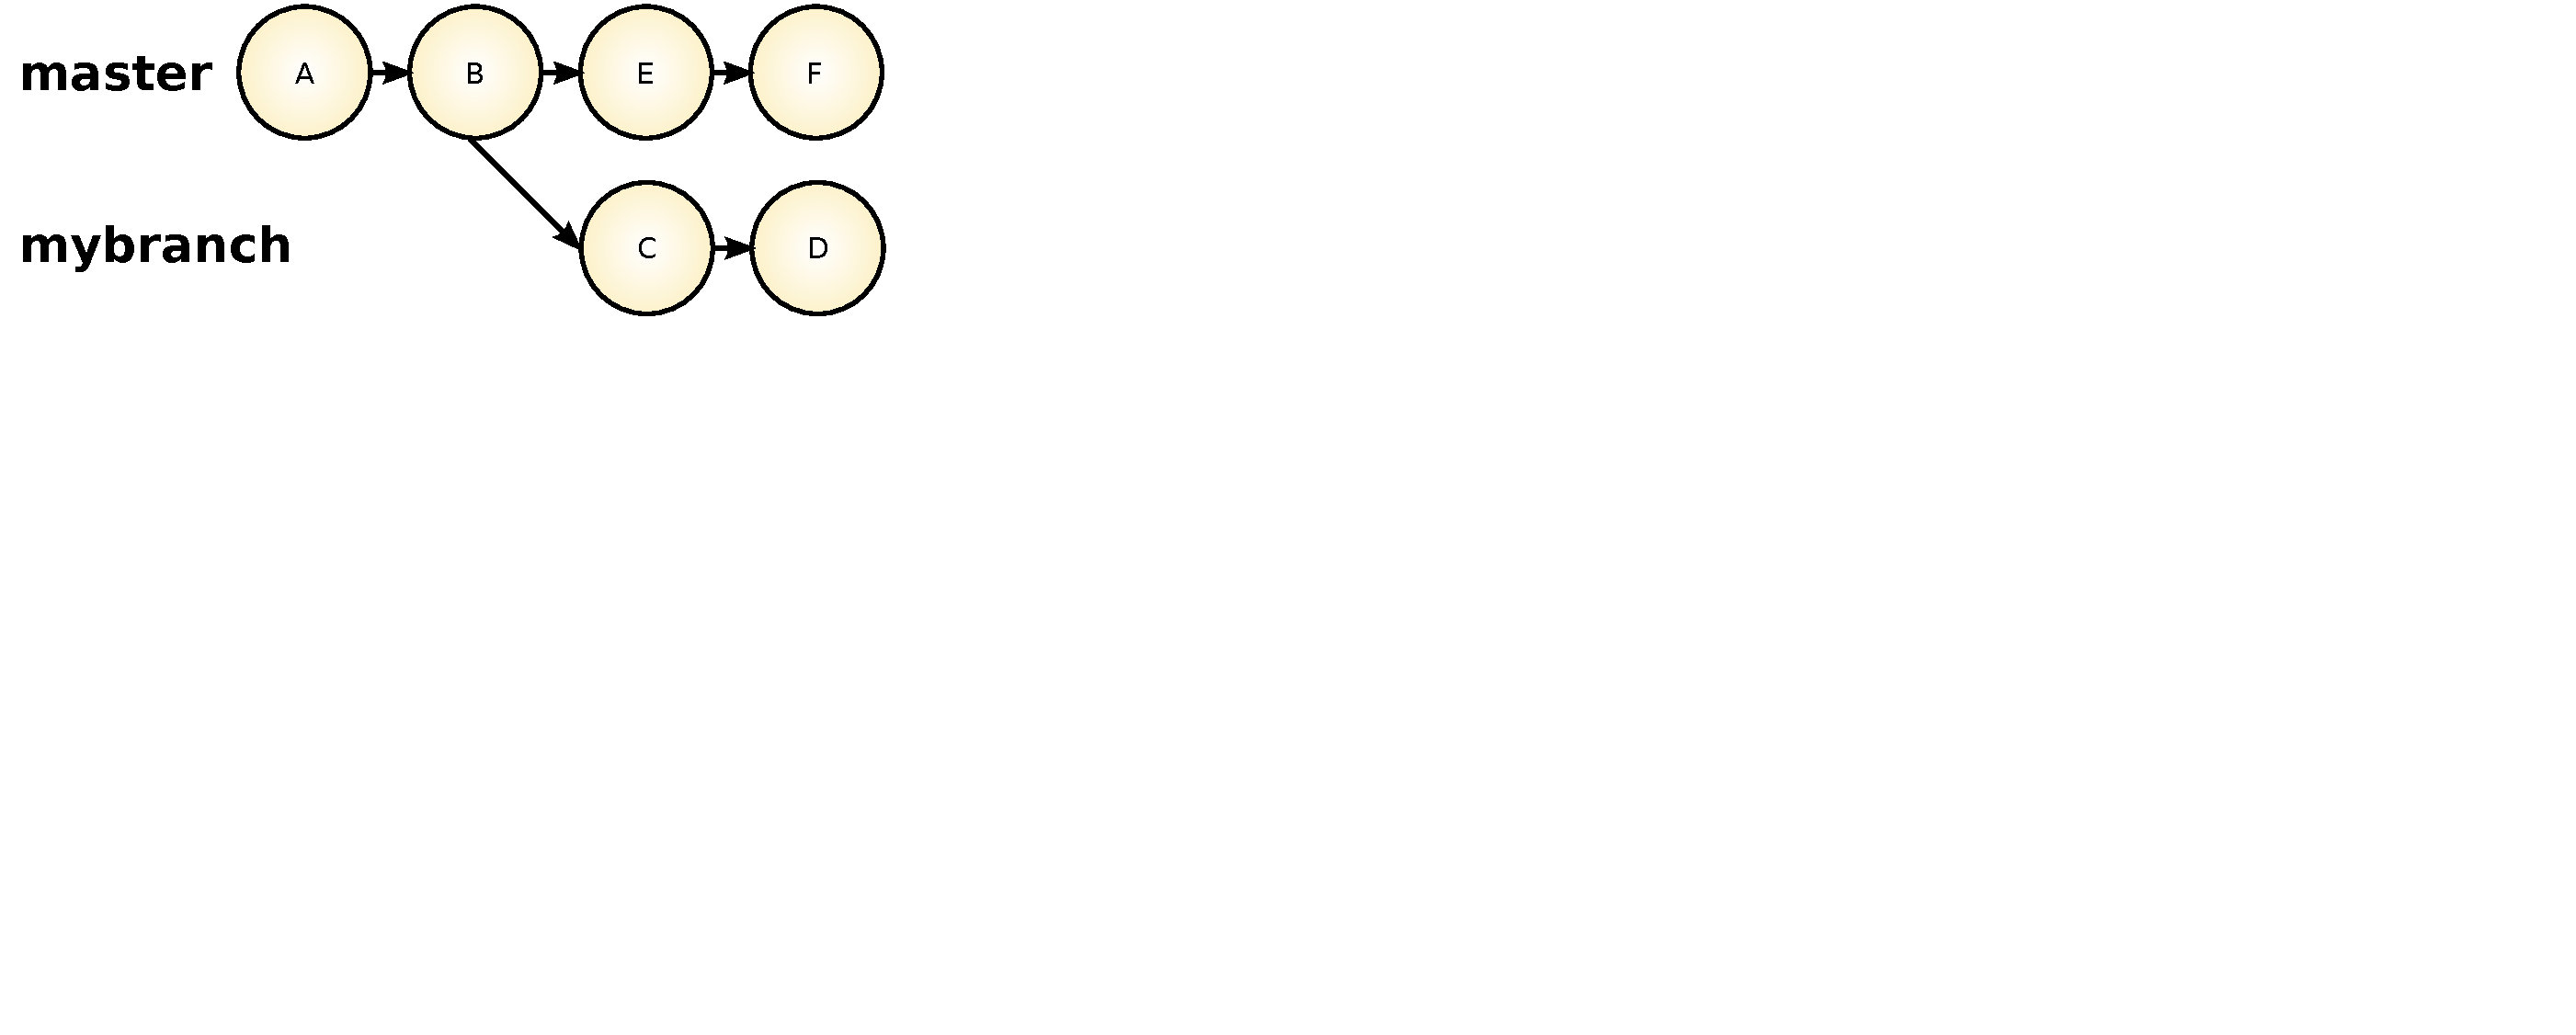
\includegraphics[width=1.00\textwidth]{images/pdf/git-rebase-1.pdf}}
    \only<3>{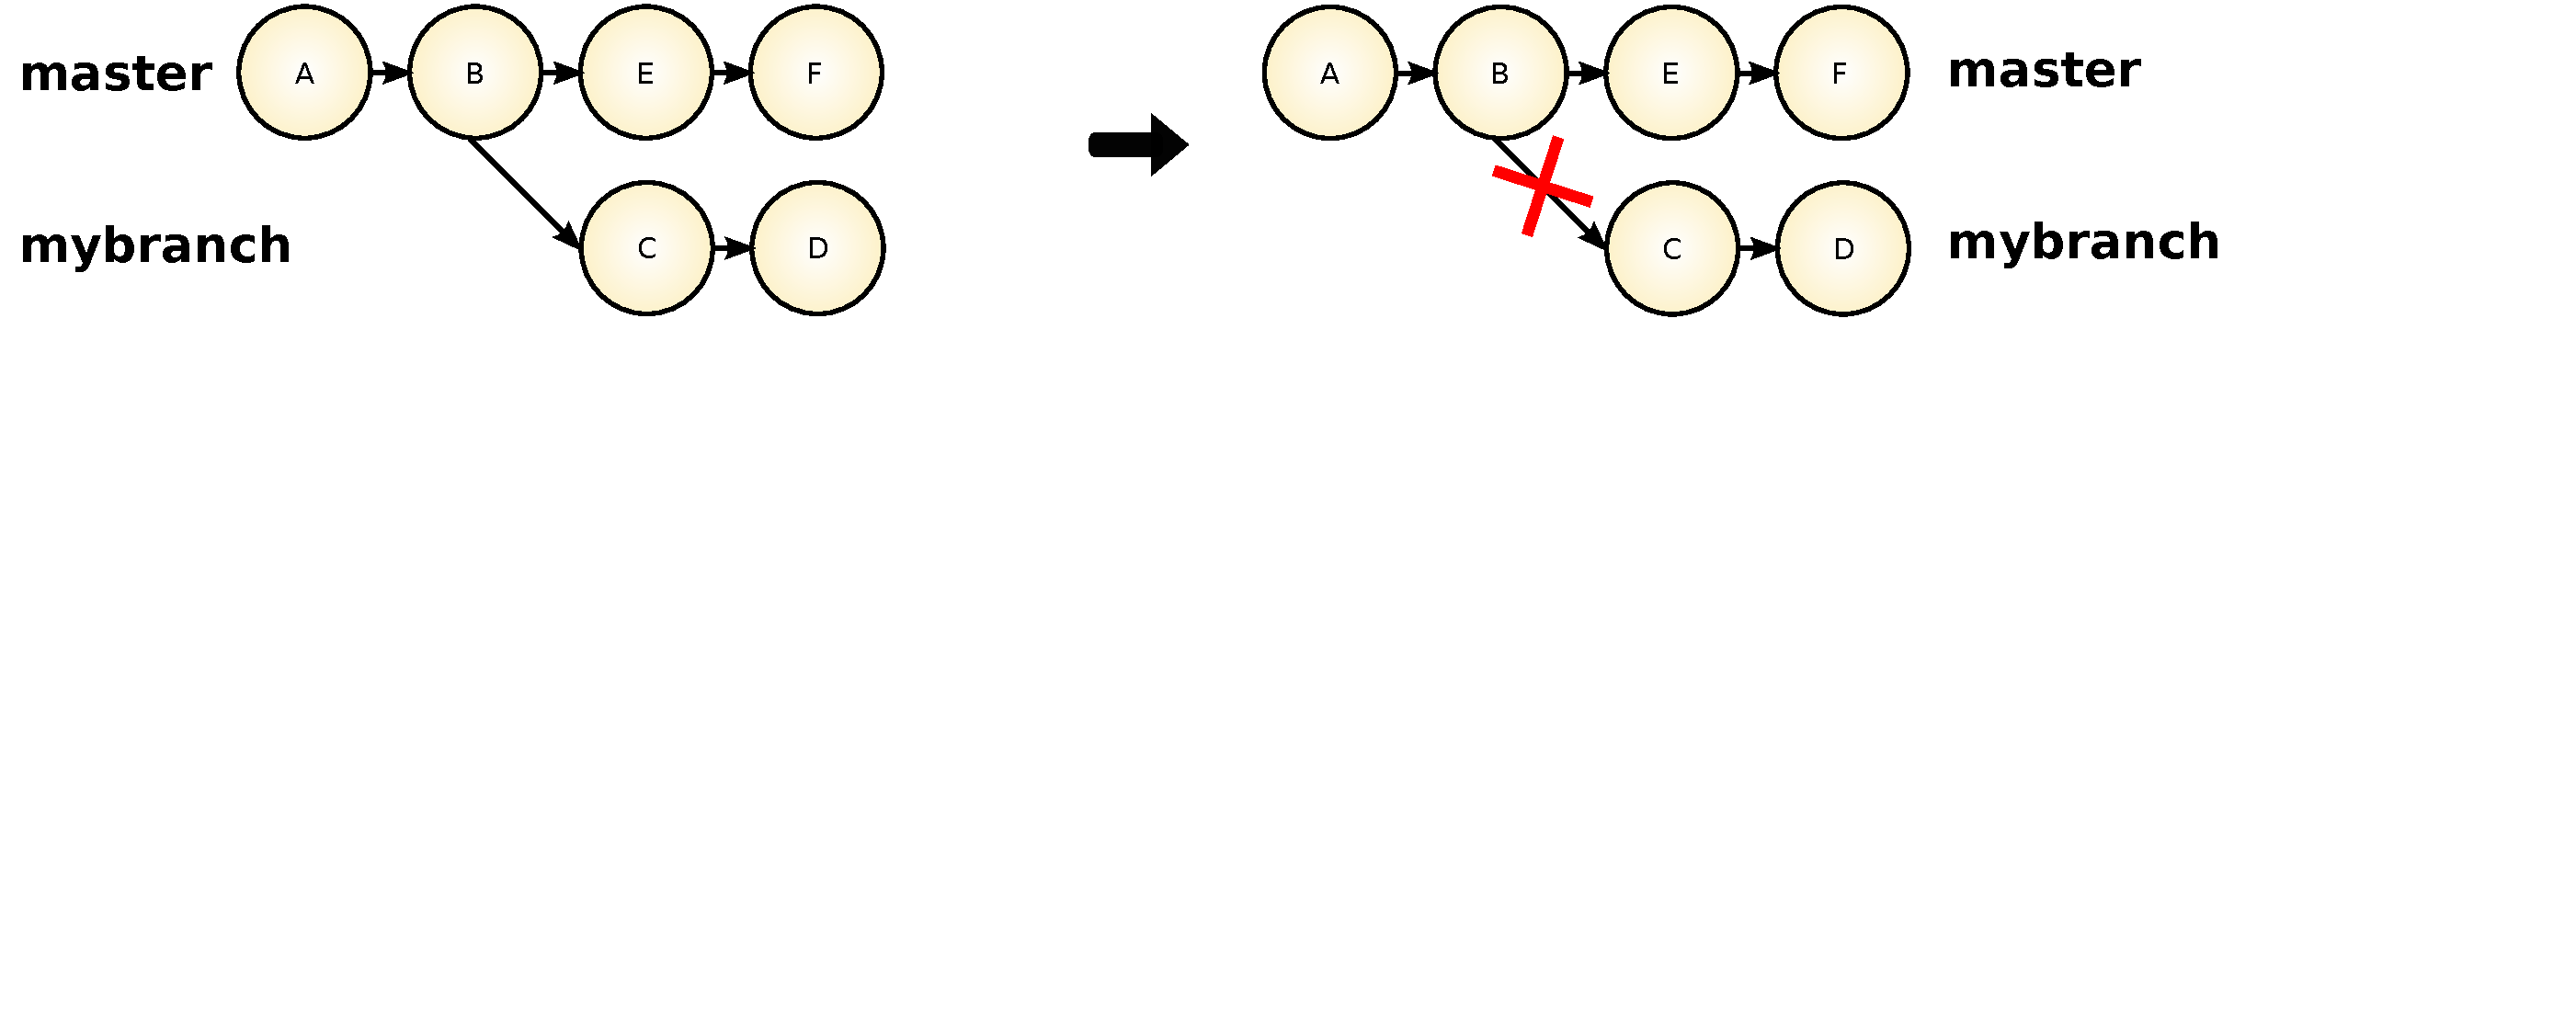
\includegraphics[width=1.00\textwidth]{images/pdf/git-rebase-2.pdf}}
    \only<4>{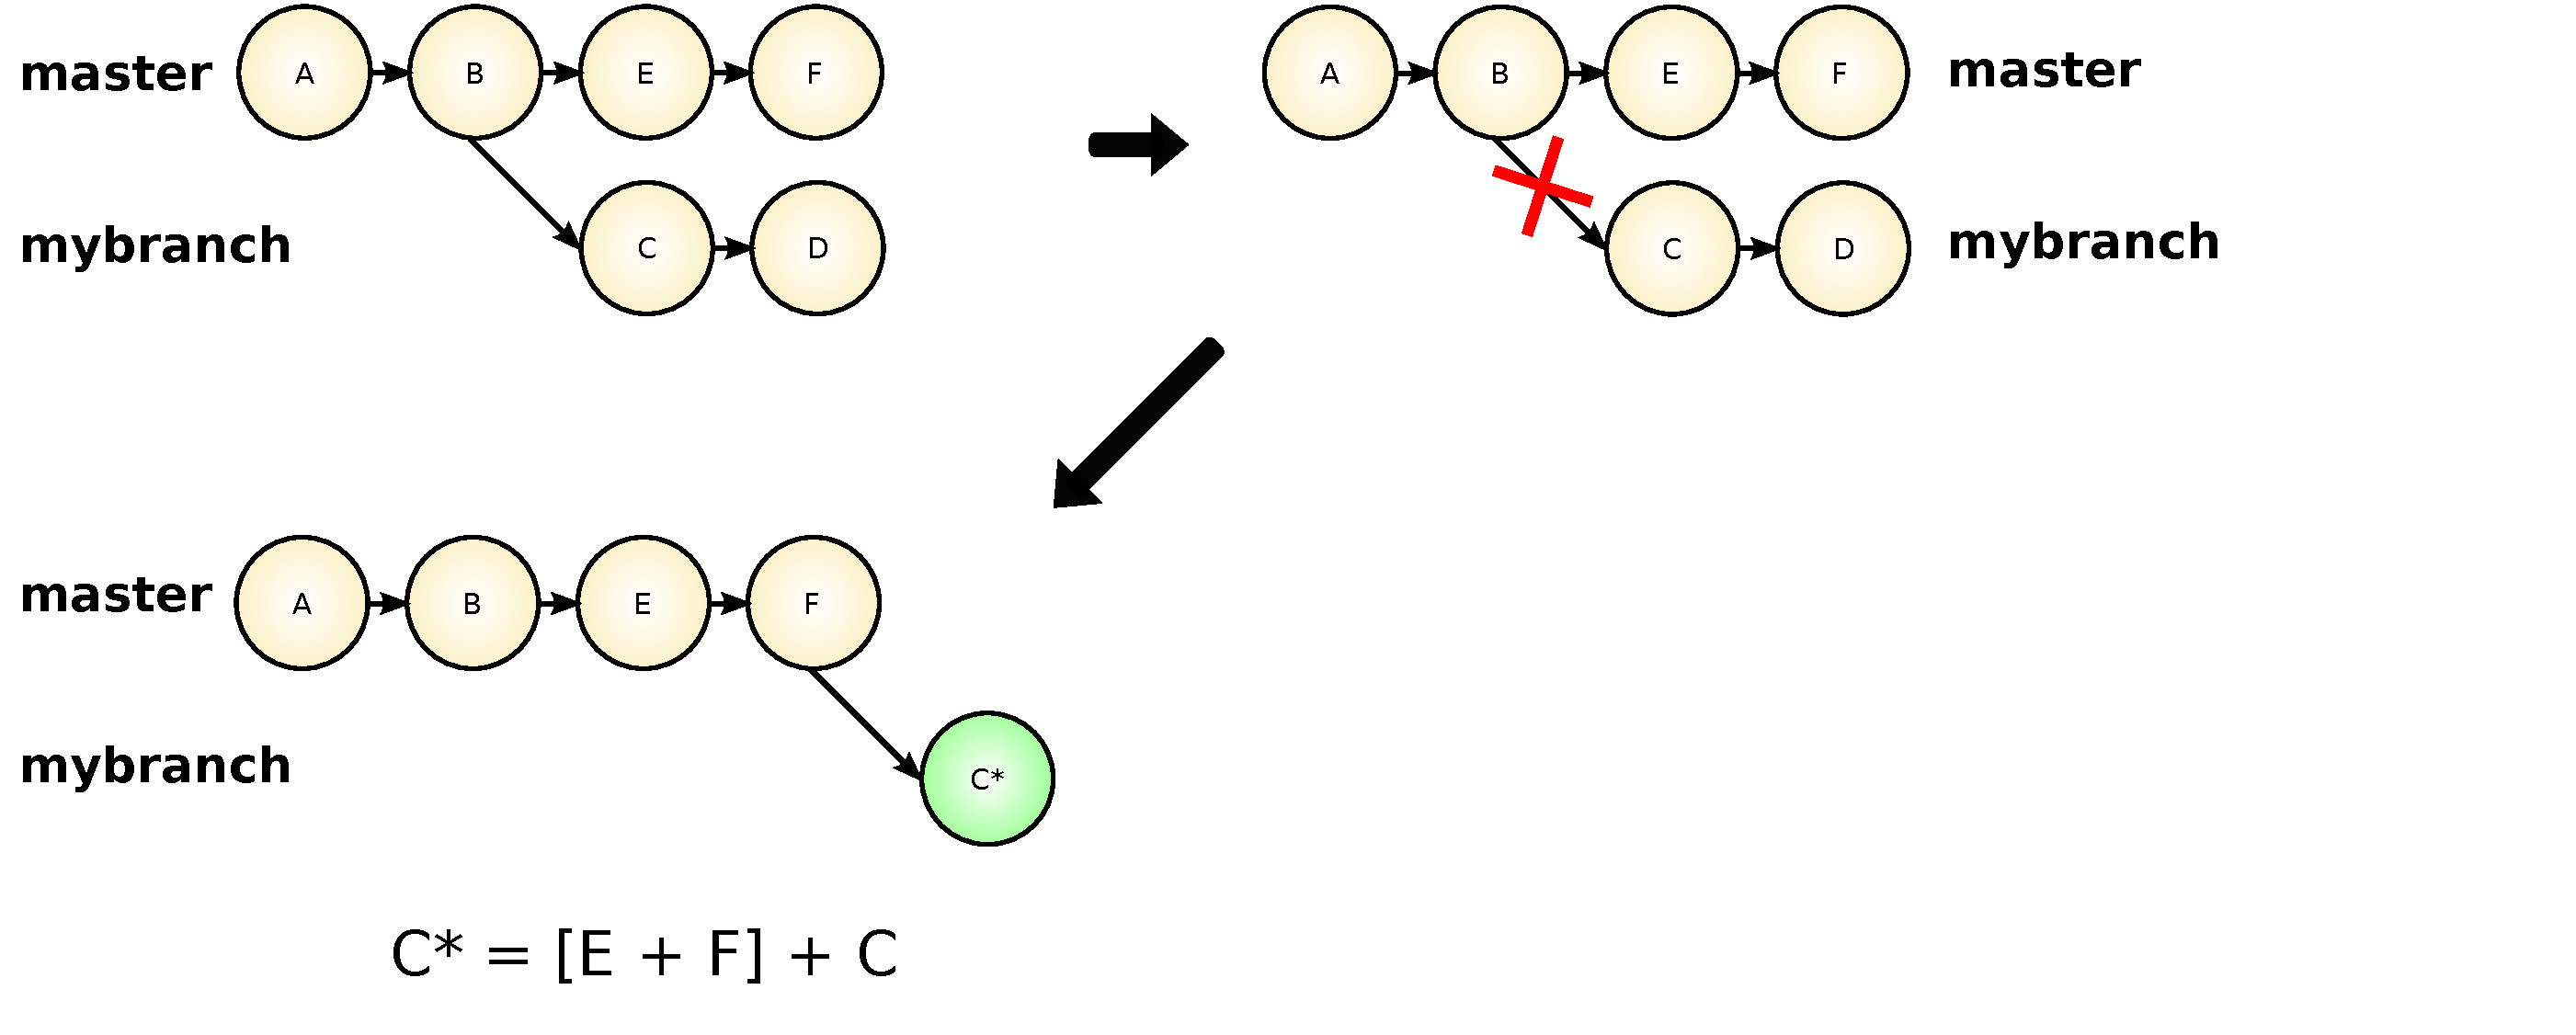
\includegraphics[width=1.00\textwidth]{images/pdf/git-rebase-3.pdf}}
    \only<5>{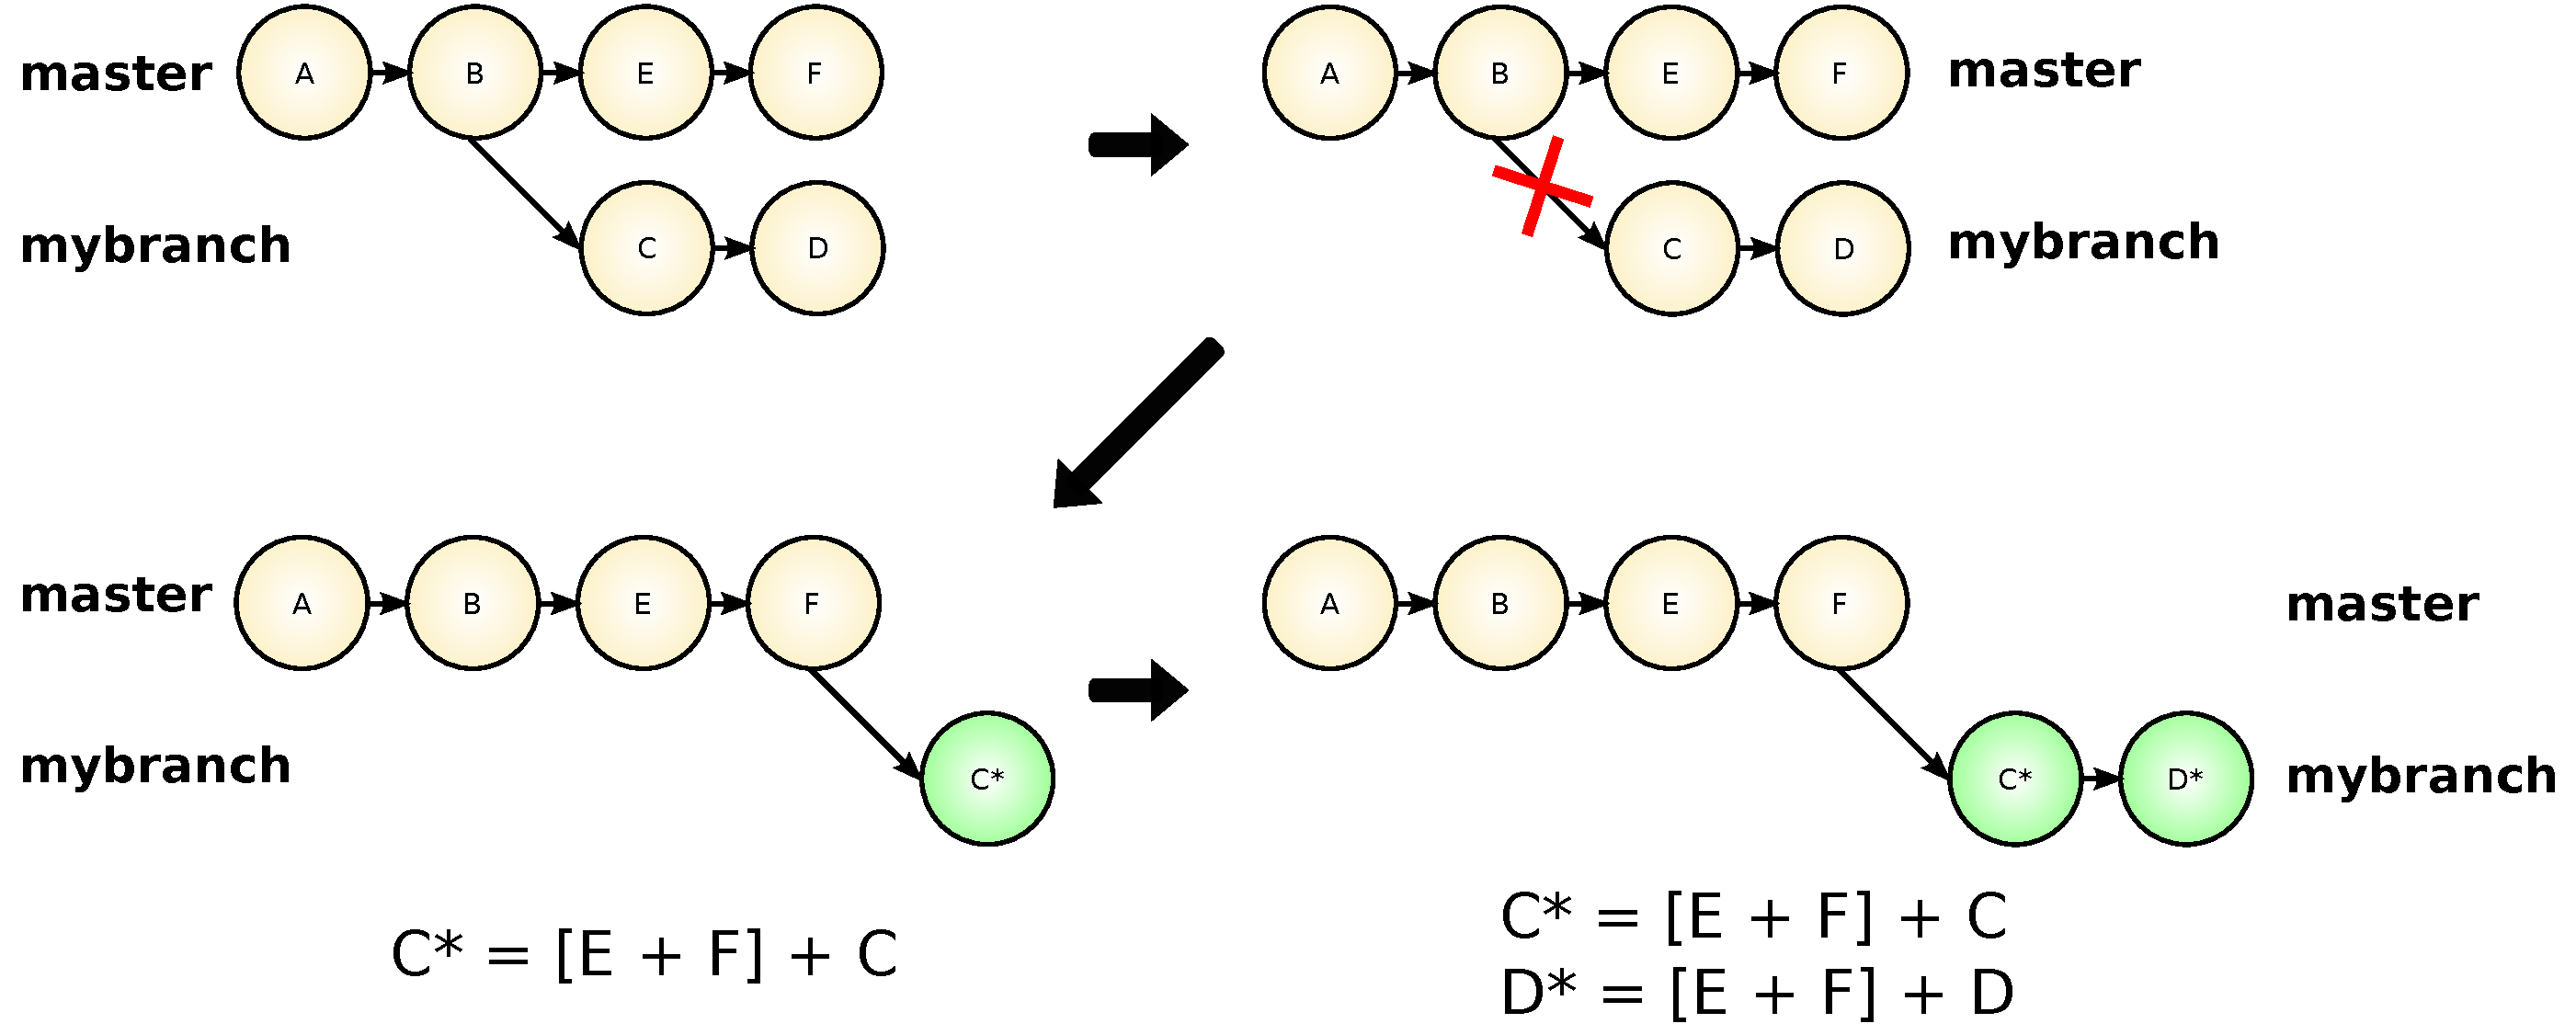
\includegraphics[width=1.00\textwidth]{images/pdf/git-rebase-4.pdf}}
  \end{center}

\end{frame}

%%%%%%%%%%%%%%%%%%%%%%%%%%

\subsection{Updating branches}

\begin{frame}[fragile]
  \frametitle{\insertsubsection}

  \vspacing
  {\Large \textbf{One personal tip} (whenever it's possible)}\\
  \vspacing Before updating a public branch with \texttt{git merge} to
  do a \texttt{git push} later on, it's a good idea to do a
  \texttt{git rebase} first from the private branch, in order to avoid
  getting a \textit{metacommit}.

  \begin{small}
\begin{verbatim}
$ git checkout mybranch # Change to private branch

$ git rebase master     # Rebase private branch

$ git checkout master   # Change back to master

$ git merge mybranch    # Merge changes from mybranch

$ git push              # Push to remote repository
\end{verbatim}
  \end{small}
\end{frame}

%%%%%%%%%%%%%%%%%%%%%%%%%%

\section{Other things...}

\subsection{Other interesting commands}
\begin{frame}
  \frametitle{\insertsubsection}

  \begin{itemize}
  \item Create a tag:\\
    \texttt{git tag <tag-name>}
    \vspacing
  \item Revert a \textit{commit} (create a new \textit{commit} on top of \textit{HEAD}):\\
    \texttt{git revert <commitID>}
    \vspacing
  \item Copy a specific commit on top of \textit{HEAD}:\\
    \texttt{git cherry-pick <commitID>}
    \vspacing
  \item Show the authors of the latest changes to a file:\\
    \texttt{git blame <filepath>}
    \vspacing
  \item Apply \textit{diff} in the \textit{Working Tree} (doesn't
    create new \textit{commits}):\\
    \texttt{git apply <diff-file>}
    \vspacing
  \item Create ``full'' patches from a given point (commit):\\
    \texttt{git format-patch <base-commitID>}
    \vspacing
  \item Apply ``full'' patches (keeping the author, log message...):\\
    \texttt{git am <patchfile>}
    \vspacing
  \end{itemize}
\end{frame}

\subsection{For further investigation}
\begin{frame}
  \frametitle{\insertsubsection}

  \begin{itemize}
  \item Save and restore temporary changes:\\
    \texttt{git stash} \& \texttt{git stash apply}
    \vspacing
  \item Modifying \textit{HEAD}, \textit{Index} and the \textit{Working Tree}:\\
    \texttt{git reset [ --soft | --hard ] <commitID>}
    \vspacing
  \item Manually rewriting the past (\textit{commits}):\\
    \begin{itemize}
    \item \texttt{git rebase -i <commitID>}
    \item \texttt{git commit --amend}
    \end{itemize}
  \item Automatically rewriting the past:\\
    \texttt{git filter-branch <params>}
    \vspacing
  \item Check out the history of git operations (and restore data):\\
    \texttt{git reflog}
    \vspacing
  \item Send patches by mail:\\
    \texttt{git send-email <email-address>}
    \vspacing
  \item Integration with \textit{Subversion} repositories:\\
    \texttt{git svn <command> [ options ] [ arguments ]}
    \vspacing
  \end{itemize}
\end{frame}

\subsection{Where to go from here}
\begin{frame}
  \frametitle{\insertsubsection}

  \begin{itemize}
  \item \textbf{\textit{Git from the bottom up} (Excellent tutorial)}:\\
    \url{http://ftp.newartisans.com/pub/git.from.bottom.up.pdf}
    \vspacing
  \item \textbf{\textit{Git User's Manual}}:\\
    \url{http://www.kernel.org/pub/software/scm/git/docs/v1.7.1/user-manual.html}
    \vspacing
  \item \textbf{\textit{Git tutorial manual page} (\texttt{man gittutorial)}}:\\
    \url{http://www.kernel.org/pub/software/scm/git/docs/v1.7.1/gittutorial.html}
    \vspacing
  \item \textbf{\textit{Everyday GIT With 20 Commands Or So}}:\\
    \url{http://www.kernel.org/pub/software/scm/git/docs/v1.7.1/everyday.html}
    \vspacing
  \item \textbf{\textit{Gitorious: infrastructure for open source projects with Git}}:\\
    \url{http://gitorious.org}
    \vspacing
  \end{itemize}
\end{frame}

